\chapter{Surrogate Assisted Bilevel Algorithm}
\label{chapter_4_sabla}



\begin{tcolorbox}
\textit{The work presented in this chapter has been published in the following article:}
\small
\begin{itemize}
\item \textbf{Islam,~M.~M.}, {Singh,~H.~K.}, and {Ray,~T.}, ``A Surrogate Assisted Approach for Single-objective Bilevel Optimization,'' {\em IEEE Transactions on Evolutionary Computation }, In Press, 2016 \textbf{(Impact factor:5.906)}.
\end{itemize}
\end{tcolorbox}


\section{Introduction}
\IEEEPARstart{F}{or} many complex real-world optimization problems, evaluating a solution involves running a computationally expensive simulation model. For example, running a computational fluid dynamics (CFD) model to evaluate an engineering design can easily take several hours on a powerful parallel computer. On the other hand, it is usually possible to stop a simulation run early, resulting in a fitness estimate with a lower accuracy (lower fidelity) and potential bias, but at much lower computational cost. Using evaluation models of different accuracy is often referred to as multi-fidelity optimization, where the term "fidelity" denotes the extent to which a model is able to mimic the behavior of the actual physical system.

In this paper, we propose a new way to make use of the possibility to prematurely stop a computationally expensive simulation run used to evaluate an individual during evolutionary optimization. The key idea thereby is to estimate the benefit a longer simulation run would have on the selection process. More specifically, we predict the probability that an individual that would be selected to survive to the next generation based on a given fidelity level, would not survive based on the highest fidelity level. If this probability of reversal is low enough, simulation is stopped. Otherwise, it is continued to the next higher fidelity level.
To the best of our knowledge, this constitutes the first paper to develop a classifier-based model management strategy to learn which of multiple (more than 2) fidelity levels should be used to evaluate individuals during evolutionary optimization.

To test our approach, we propose two new benchmark problems, one artificial and one based on real CFD simulation data on the design of a toy submarine. Based on these benchmark problems, we analyze the workings of our algorithm and demonstrate that it is capable of outperforming alternative approaches over a range of computational budgets. 

%Do we only consider models where a higher fidelity model is a continuation of a lower fidelity model, or can it any fidelity model (in which case running f2 may be more expensive than running f1)?
%Probably we leave CFD iterations for the ASME paper?

The paper is structured as follows. Related work is surveyed in Section~\ref{sec:related}. The new approach is described in Section~\ref{sec:MFEA}, followed by a description of the proposed benchmark problems in Section~\ref{sec:benchmarks} and an empirical evaluation in Section~\ref{sec:results}. The paper concludes with a summary and some ideas for future work.

\section{Related work\label{sec:related}}

The challenge of expensive fitness evaluations can be addressed in different ways, most notably by parallelization (e.g., \cite{GCZZZ15}) or by using approximate, faster to compute surrogate fitness functions (e.g., \cite{Bhatt13}).
In this section we only deal with the latter, and discuss evolutionary approaches involving fitness approximations in Subsection~\ref{sec:evoSurrogate}, whereas some non-evolutionary approaches using partially converged CFD simulations are discussed in Subsection~\ref{sec:nonEA}.

\subsection{Evolutionary Optimization Using Surrogate Models \label{sec:evoSurrogate}}
The use of approximate fitness models within an evolutionary algorithm (EA) for computationally expensive fitness functions has been investigated in numerous papers, and comprehensive surveys 
can be found in  \cite{JinBranke2005,Jin2005,Jin2011,Shi2010}.

In most cases, a surrogate model is learned over the course of the run from fully evaluated solutions (e.g., \cite{BeKe01,Emmerich2002,Lim2010}), but there are also a few papers that assume a given set of different fidelity models (e.g., \cite{EAPG98}). One key difference is that a learned model usually aims at predicting the exact fitness values and the prediction improves as more data is collected. Different types of models can be used for learning, from simple fitness inheritance \cite{SGP01} over regression \cite{BrSc05} to Artificial Neural Networks \cite{Jin2002} or Gaussian Processes \cite{BeKe01,LZG14}. Usually, the models require a distance metric between genotypes. A phenotypic similarity measure that allows using surrogate models also in combination with Genetic Programming has recently been proposed in \cite{HiBr15}.
In typical multi-fidelity problems such as partially converged CFD simulations, the surrogate models are given and static, and the fitness values generated from the lower fidelity models may be expected to have some correlation with the highest fidelity model, but are not necessarily a good predictor.

In any case, a key challenge is to decide which individuals are to be evaluated by the surrogate model, and which are to be evaluated by the exact model, an issue often called "meta-model management" \cite{GJS07}. Different categories can be identified. In generation-based approaches, the same model is used for all individuals within a generation, but the model is switched between generations, whereas in individual-based approaches, decisions about which model to use have to be made for each individual \cite{Jin2005}. Some papers use surrogate models only for locally improving an individual, in which case model management techniques developed in the engineering community such as the trust-region based approach can be used \cite{ONK03,ZOL07,Zhou2007}. 
A theoretical investigation of the influence of a lower-fidelity surrogate on a $(1+1)$-EA can be found in~\cite{CXZ13}.
In the following discussion, we will focus on a subset of papers most relevant to our approach, e.g. because they are adaptive or use more than one surrogate model. 

A commonly used individual-based model management scheme is that of pre-selection \cite{USZ04,Emmerich2002}. With pre-selection, in each generation, a larger set of individuals is evaluated with the surrogate model, and only the best subset is then re-evaluated using the exact fitness function. In \cite{USZ04},  a $(\mu,\lambda)$-ES is considered. 
In every generation, $\lambda_{pre} > \lambda$ offspring are generated out of which $\lambda$ are pre-selected using the surrogate model.
The paper proposes adjusting the size $\lambda_{pre}$ over time depending on how accurate the surrogate model would be in selecting $\mu$ out of the $\lambda$ individuals. 
%$\lambda_{pre}$ is increased if the surrogate model would do better than random on selecting the $\mu$ parents among the $\lambda$ offspring, and is reduced otherwise. 
While the authors report good results with this approach, \cite{GJS07} compares a number of adaptation strategies for $\lambda_{pre}$ and finds that none of them is able to significantly outperform the approach with a fixed $\lambda_{pre}$.

Some surrogate models such as kriging provide an accuracy estimate along with the fitness estimate. This has been exploited for example in \cite{BeKe01,BrSc05} who suggest re-evaluating solutions where the surrogate model is less certain. Emmerich et al.\cite{Emmerich2002} propose the pre-selection idea not based on estimated fitness, but estimated fitness plus standard deviation, i.e., giving higher preference to individuals for which the kriging model predicts higher uncertainty. In \cite{Zhou2007}, the probability of improvement criterion is used for pre-selection.

Runarsson \cite{Runarsson04} suggested an adaptive approach where the high fidelity model is only used to evaluate a small subset of the $\lambda$ solutions which are best according to the low fidelity model, but additional solutions are evaluated if an update of the model with the new information changes its ranking prediction of the $\lambda$ individuals.

Ziegler and Banzhaf\cite{ZiBa03} propose learning a classifier based on genotypic information to decide, for the case of tournament selection, which of the two individuals is the better one. If the classifier is "confident enough", the decision is made. Otherwise, the two individuals are evaluated with the high fidelity model. A similar idea is used in \cite{TaSa08} for Differential Evolution. When deciding whether a child should be evaluated with the high fidelity model, the uncertainty of the model and the fitness difference between the child and its parent are used to identify child individuals that are clearly worse. If the child can not be discarded based on the surrogate model, it is evaluated with the high fidelity model. In \cite{TaSa10}, an adaptation mechanism for the threshold that is used to discard child individuals is suggested, based on the percentage of children surviving to the next generation. 

Only few approaches employ more than two models. 
In \cite{Le2013}, an "evolvability measure" is proposed that estimates the expected fitness improvement if local search is done with a particular surrogate modeling approach. This measure is then used to select the most suitable surrogate model. Tenne~\cite{Tenne2013} proposes a framework in which the algorithm to construct surrogate models as well as the search algorithm is adapted online during the run.

Ray et al.\cite{RTT02} vary the granularity of the mesh from coarse to fine at pre-defined stages over the run of the EA.
In, \cite{EAPG98}, an island-EA is used, where each island runs an EA with a different fidelity level, and occasionally the best found individuals are exchanged (and re-evaluated at the receiving island). A similar idea was proposed also in \cite{SePe00} and \cite{KaGi08}.
In \cite{BeKe99}, three different ways to use multi-fidelity models in evolutionary computation have been compared: Progressive, i.e., starting with the lowest fidelity model then moving towards more complex models in later generations; full mixing, where in every generation a certain percentage of the evaluations is done with each fidelity, and gradual mixing, where the proportion of individuals evaluated with different fidelity models is adapted over time, with higher percentages of higher fidelity evaluations in later generations. For testing, they use a modified bump function with two additional parameters to modify the frequency of bumps and to shift the function. Testing many different algorithms with these schemes, they observed relatively small benefits compared to simply always using the highest fidelity model, but concluded that the progressive model works best.

We are aware of only one other paper that explicitly uses partially converged CFD simulations.
Lim et al.~\cite{Lim2008}  use a lower fidelity model to locally optimize each solution in the population. The fidelity used is decided based on a user defined threshold $\eta$ that specifies the minimum correlation required between the model chosen and the highest fidelity model. All fully evaluated solutions are stored in a database. For a particular solution $x$, the $m$ nearest neighbors are retrieved and the correlation between fidelity model $i$ and the highest fidelity model for these solutions is computed. Then, the lowest fidelity model with sufficiently high correlation is chosen for local optimization. The locally optimized solution $x'$ is then re-evaluated using the highest fidelity model and replaces $x$ if it is better. \cite{BraHil14} optimize dispatching rules for on-line scheduling and abort the simulation and assign the individual a very poor fitness if the work-in-process exceeds sustainable levels.

Compared to previous work on surrogate-based evolutionary computation, the present paper is the first to develop a classifier-based model management strategy for the use of multi (more than two) fidelity models.

\subsection{Non-evolutionary Optimization Using Partially Converged CFD Simulations \label{sec:nonEA}}
There are also a number of papers related to our work that are not based on evolutionary computation.
Forrester et al.~\cite{FBK03} examine the use of partially converged CFD simulations in response surface optimization. They suggest three ways how partially converged data can be used. First, search a response surface constructed with partially converged data to find points with maximum expected improvement. These points are then fully evaluated to build the final response surface model used for optimization. Second, the response surface model (RSM) based on partially converged data is used to reduce the search space to an area around the observed optimum. Only the data points in the reduced space are now fully evaluated and used to construct the final RSM on the restricted search space.
Third, the RSM search is done based on partially converged data, and only the final solution is fully evaluated. They conclude that the first method offers the best compromise between speed and accuracy. 

In \cite{FBK06}, a method called "evofusion" is proposed which starts with constructing a low fidelity surrogate model (in this case based on partially converged CFD simulations). It then iteratively samples new data points (e.g. according to largest expected improvement criteria), evaluates them with a fully converged simulation, and from the difference calculates an error model that can be used to correct the output of the low fidelity model. The paper also discusses a way to decide on the size and iteration number for the initial DoE to build the low fidelity model, based on the stability of the model when size and iteration number are increased. A more recent sequential kriging optimization method based on multi-fidelity information can be found in \cite{GrCa15}.

Cao et al.\cite{CJKS08} attempt to predict the result of a fully converged CFD run based on results of a partially converged run using a differential recurrent neural network and mention that this idea could be integrated into an optimization algorithm.




\section{Managing partially converged CFD simulations in evolutionary optimization\label{sec:MFEA}}

In the following subsection, we describe our proposed EA for multi-fidelity optimisation (MFEA), followed by a small worked example and a discussion of a particular aspect called "forcing".

\subsection{Multi-fidelity Evolutionary Algorithm (MFEA)}
Evolutionary algorithms need accurate fitness evaluations that allow them to correctly apply Darwin's principle of survival of the fittest and select the better individuals to survive and reproduce. However, as for example noted in \cite{SBC06,Runarsson04}, not all fitness values need to be equally accurate, and the required accuracy depends on the distribution of fitness values and the selection mechanism used.
For example, most modern EAs today use rank-based selection, which means that not the absolute fitness values are important, but only the ranking.

In our paper, we assume a $(\mu+\lambda)$-EA. In this case, all that is important in terms of survival is whether a particular solution falls into the top $\mu$ individuals (and should survive to the next generation) or not (and should be discarded).
If the information from a low fidelity model is sufficient to confidently classify an individual into one or the other category, then a more accurate evaluation will only use up additional computational effort without improving the selection decision.

So, the main idea of this paper is to learn the probability that the classification of an individual based on the evaluation with a given fidelity level is wrong. If this probability is above a pre-defined threshold $\delta$, the individual is evaluated also with the next higher fidelity level. Otherwise, the classification is assumed to be correct.
For this idea to work efficiently, we assume that it is possible to save the state of a simulation run, and continue it at a later time if needed. That way, if a CFD simulation of a particular individual has been performed up to a certain fidelity level~$i$, and later it seems necessary to evaluate the individual at fidelity level $j>i$, then only the cost difference between fidelity level $j$ and fidelity level~$i$ is incurred at that stage.

We base our estimated probability estimate on a simple pairwise comparison between individuals. Let $f^i(x)$ denote the fitness of individual $x$ in fidelity level $i$, where $i=1$ is the lowest fidelity level and $i=M$ is the highest fidelity level. Then we want to learn the probability that the ranking of two individuals $x$ and $y$ based on a particular fidelity level $i$ is inconsistent with the ranking these two individuals would see when evaluated on the highest fidelity level, i.e., 
\begin{eqnarray}
P(f^M(x)>f^M(y))|f^i(x)<f^i(y)).
\end{eqnarray}

To estimate this probability of reversal, we use a logistic regression model for each fidelity level $i$, $\mbox{LR}^i(\Delta f^i)$, that returns a probability depending on the fitness difference on fidelity level~$i$, $\Delta f^i =|f^i(x)-f^i(y)|$. The logistic regression model is based on all the data of fully evaluated individuals over the run so far. We chose logistic regression as predictor because it seems sensible to assume that the probability of reversal increases with increasing fitness difference, and logistic regression naturally incorporates this monotonicity. Furthermore, there exists a fitness difference $\Delta_c$ such that $\mbox{LR}(\Delta)<\delta$ for all $\Delta > \Delta_c$, i.e., our expected probability of rank reversal is below the allowable threshold $\delta$ if the fitness difference is larger than $\Delta_c$. 

%We learn these probabilities during the run based on previously fully evaluated solutions. The input to our predictor is the absolute fitness difference between solutions $x$ and $y$ on fitness level $i$, $|f^i(x)-f^i(y)|$, and the output being the probability of rank reversal (i.e., the probability that the individual evaluated better on fidelity level $i$ is actually worse based on fidelity level $M$). Because it seems sensible to assume that the probability of reversal increases with increasing fitness difference, we chose a logistic regression model as predictor.
%Let us denote the resulting predictor of rank reversal for fidelity level $i$, $R^i(\Delta f^i)$. Because $R$ is determined by logistic regression, there exists a fitness difference $\Delta_c$ such that $R(\Delta)<\delta$ for all $\Delta > \Delta_c$, i.e., our expected probability of rank reversal is below the allowable threshold $\delta$ if the fitness difference is larger than $\Delta_c$. 

During the selection step, we iterate through the fidelity levels from lowest fidelity to highest fidelity and make selection decisions where we are confident, or re-evaluate at a higher fidelity level where we are not.

First, all individuals are evaluated and ranked on the lowest fidelity level. Let $x_{(k)}$ denote the individual with rank $k$ on this fidelity level. If the goal is to select the best $\mu$ individuals from the population, then from this ranking, we determine a fidelity~1 fitness threshold $T^1=f^1(x_{(\mu)})$ which is the fitness of the worst individual still included in the next population (rank $\mu$). Now we consider all individuals for which the current fidelity is the highest evaluated fidelity. We compare their fitness with this fitness threshold and estimate the probability of being better or worse. For example, for an individual $x$ ranked better than (smaller predicted fitness for minimization problems) the threshold $T$, the estimated probability of incorrect selection (i.e., of not being among the top $\mu$ individuals at highest fidelity level) would be $\mbox{LR}^1(T^1-f^1(x))$. If this probability is below a pre-defined probability threshold, the individual would be accepted on this fidelity level, otherwise it would be marked as undecided. Similarly, for an individual not ranked among the top $\mu$, we would calculate $\mbox{LR}^1(f^1(x)-T^1)$ and discard the individual if this value is below the probability threshold, and mark it as undecided otherwise.
At the end of the iteration, all individuals marked "undecided" are evaluated with the next higher fidelity level (unless these values are already known from previous iterations in which case they are simply copied over).
Then, we repeat the process on the next fidelity level but only with the individuals that have an evaluation on this fidelity level.

The complete procedure is summarized in Alg.~\ref{alg:MFEA}.

\begin{algorithm}[!htb]\scriptsize
	\caption{MFEA\label{alg:MFEA}}
	\textbf{Input:} $\mu$ = Population size, $FE_{max}=$ Total computational budget, $\delta$ = Allowed probability of rank reversal, $FES$ = Forced evaluation strategy, $M$ = Number of fidelity levels, $C_f = $Evaluation cost in each fidelity level $f=1,2.....M $\\\\
	\begin{algorithmic}[1]
		\STATE $FE=0, Gen=0$
		\STATE Initialize~($pop$) \COMMENT {Population of $\mu$ individuals}
		\STATE Evaluate$^{1:M}(pop)$ \COMMENT {Evaluate initial pop for all fidelity levels}
		\STATE $pop_{1:\mu,currgen}=Gen$ \COMMENT{last generation individual was evaluated}   
		\STATE Update($FE$)   
		\WHILE{$(FE < FE_{max})$}
		\STATE $Gen=Gen+1$
		\STATE Build Logistic Regression Models; 
		\STATE $childpop$ = Generate $\mu$ unique child solutions 
		\STATE Evaluate$^1(childpop)$ \COMMENT{Evaluate all children on $f^1$}
		\STATE $f^{2:M}(childpop_{1:\mu})=NaN$ \COMMENT{Other fidelity levels not yet evaluated}
		\STATE $childpop_{1:\mu,currgen}=Gen$
		\STATE Replace all $\pm inf$ in $pop_{1:\mu,f^{2-M}}$ by $NaN$ \COMMENT{Initialisation}
		\STATE $S=pop+childpop$
		\FOR{$\textit{j = 2:M}$}  %FOR j
		\STATE Sort$(S,f^{j-1})$ \COMMENT{Sort $S$ according to fidelity level $j-1$}
		\STATE $T^{j-1} = f^{j-1}(S_{\mu})$ \COMMENT{Compute selection threshold $T$} 
		\FOR {$i=1:2\mu$}              %FOR i
		%\COMMENT {Loop through all individuals}
		\IF {$(f^{j}(S_{i})=NaN)$} %IF1
		\IF{$(\mbox{LR}^{j-1}(|f^{j-1}(S_{i})-T^{j-1}|)<\delta)$} %IF2
		\IF {$i\leq \mu$}  %IF3
		\STATE $f^{j:M}(S_i)=-Inf$ \COMMENT{Keep for sure} 
		\ELSE
		\STATE $f^{j:M}(S_{i})=Inf$ \COMMENT{Discard for sure}
		\ENDIF  %IF3
		\ELSE
		\STATE Evaluate$^j(S_{i})$ 
		%			 \STATE $S_{i,currgen}=Gen$
		\ENDIF %IF2
		%                \ELSIF{$(f^{j}(S_{i})=-Inf)$}
		%                   \IF {$(S_{i,currgen} \neq Gen)$ \& (FES = 1)} %\COMMENT{Forcing}
		%                 	 \STATE Evaluate$^j(S_{i})$ 
		%			 \STATE $S_{i,currgen}=Gen$
		%                \ENDIF %IF4
		\ENDIF %IF1 
		\STATE Update($FE$) 
		\IF {($size(f^j(S_{1:2\mu})=-Inf) = \mu$)}
		\STATE Replace all $NaN$ in $S_{\mu+1:2\mu,f^{j+1:M}}$ by $Inf$
		\STATE \textit{\textbf{break to line 39}}
		\ELSIF {($size(f^j(S_{1:2\mu})=Inf) = \mu$)}
		\STATE Replace all $NaN$ in $S_{1:\mu,f^{j+1:M}}$ by $-Inf$
		\STATE \textit{\textbf{break to line 39}}
		\ENDIF
		\ENDFOR
		\ENDFOR
		\STATE Forcing of one individual up to highest fidelity level
		\STATE Sort $(S)$
		\STATE $pop=S_{1:\mu}$
		\ENDWHILE
	\end{algorithmic}
	\label{alg:MFEA}
\end{algorithm}


\subsection{Worked example}
Let us consider a simple example with $\mu=\lambda=3$ and $M=4$. Table~\ref{tab:ex1} shows the information available in the first stage of the algorithm, after all three children (denoted $x_4, x_5, x_6$) have been evaluated on the lowest fidelity level (fitnesses are in bold face to indicate they have just been evaluated at this fidelity level). The parent individuals $(x_1, x_2, x_3)$ have been evaluated at higher fidelity levels in previous generations. First, individuals are sorted according to $f^1$. Based on $f^1$, individuals $x_1, x_3$ and $x_6$ would be accepted, the others discarded. The quality threshold is $T^1=f^1(x_6)=7$. Now let us assume that our logistic regression model predicts that with a fitness difference of more than $\Delta_c^1=1.9$, the probability for rank reversal is sufficiently low to be confident in the ranking. This means that solutions with $f^1<T^1-\Delta_c^1=5.1$ could be safely accepted, and solutions with $f^1>T^1+\Delta_c=8.9$ could be safely discarded. In our case, this means $x_1$ could be accepted, but since we already have higher fidelity evaluations, the solution is simply kept in the race. Solution $x_5$ on the other hand is permanently discarded at this point, which is recorded as a fitness of $\infty$ on all higher fitness levels. Solutions $x_6$ and $x_4$ are re-evaluated on fidelity level~2, as they can be neither safely accepted nor safely discarded.

This then results in the information depicted in Table~\ref{tab:ex2}. Note that the table is now sorted according to fidelity level 2, and $x_3$ is the new best individual. $T^2=5.6$ and assume $\Delta_c^2=1$. In this case, $x_1$ can be safely accepted (receiving fitness $-\infty$ on higher fitness levels), whereas solutions $x_4$ and $x_6$ need to be evaluated on fidelity level~3, resulting in Table~\ref{tab:ex3}. Finally, on fidelity level~3, $T^3=5$ and with $\Delta_c^3$=0.4, solutions $x_2$ and $x_6$ can be safely discarded, whereas $x_4$ needs another evaluation at fidelity level 4. Then, the algorithm stops and simply picks the best solutions according to fidelity level~4 in the final summary Table~\ref{tab:ex4}, i.e., solutions $x_1, x_4,$ and $x_3$.

\begin{table}
	\caption{Example of the information available just after all offspring has been evaluated at fidelity level 1. $T^1=7$, and assume $\Delta_c^1=1.9$. \label{tab:ex1}}
	\begin{center}
		\begin{tabular}{c|cccc}
			%&\multicolumn{4}{c}{fidelity level}\\
			Ind.&$f^1$&$f^2$&$f^3$&$f^4$\\ \hline
			$x_1$&5&4.5&&\\
			$x_3$&6&4.4&4.2&4.1\\
			$x_6$&{\bf 7}&&&\\
			$x_4$&{\bf 8}&&&\\
			$x_2$&8.5&7&6&\\
			$x_5$&{\bf 10}&&&\\
		\end{tabular}
	\end{center}
\end{table}

\begin{table}
	\caption{Example of the information available at stage 2 of the algorithm. $T^2=5.6$, and assume $\Delta_c^2=1$. \label{tab:ex2}}
	\begin{center}
		\begin{tabular}{c|ccc}
			%&\multicolumn{4}{c}{fidelity level}\\
			Ind.&$f^2$&$f^3$&$f^4$\\ \hline
			$x_3$&4.4&4.2&4.1\\
			$x_1$&4.5&&\\
			$x_4$&{\bf 5.6}&&\\
			$x_6$&{\bf 5.8}&&\\
			$x_2$&7&6&\\
			$x_5$&$\infty$&$\infty$&$\infty$\\
		\end{tabular}
	\end{center}
\end{table}

\begin{table}
	\caption{Example of the information available at stage 3 of the algorithm. $T^1=5$, and assume $\Delta_c=0.4$. \label{tab:ex3}}
	\begin{center}
		\begin{tabular}{c|ccc}
			%&\multicolumn{4}{c}{fidelity level}\\
			Ind.&$f^3$&$f^4$\\ \hline
			$x_1$&$-\infty$&$-\infty$\\
			$x_3$&4.2&4.1\\
			$x_4$&{\bf 5}&\\
			$x_2$&6&\\
			$x_6$&{\bf 6.1}&\\
			$x_5$&$\infty$&$\infty$\\
		\end{tabular}
	\end{center}
\end{table}

\begin{table}
	\caption{Example of the final information available for the selection process. \label{tab:ex4}}
	\begin{center}
		\begin{tabular}{c|cccc}
			%&\multicolumn{4}{c}{fidelity level}\\
			Ind.&$f^1$&$f^2$&$f^3$&$f^4$\\ \hline
			$x_1$&5&4.5&$-\infty$&$-\infty$\\
			$x_4$&8&5.6&5&4.5\\
			$x_3$&6&4.4&4.2&4.1\\
			$x_6$&7&5.8&6.1&$\infty$\\
			$x_2$&9&7&6&$\infty$\\
			$x_5$&10&$\infty$&$\infty$&$\infty$\\
		\end{tabular}
	\end{center}
\end{table}

\subsection{Forcing}
Because our learning algorithm requires information about the highest fidelity level in the region of interest, and also because there is a danger that solutions perceived as excellent based on their low fidelity evaluation survive forever although they are actually quite poor with respect to the highest fidelity, we employ a method we call "forcing": 
In each generation, from the $\mu$ best solutions and ignoring the fully evaluated ones, we pick the solution with the smallest estimated probability of reversal based on its highest fidelity level evaluated, and evaluate it to the highest fidelity level. This guarantees a minimal flow of highest fidelity information that can be used to update our probability models.



\section{New benchmark problems\label{sec:benchmarks}}
In this section, we propose two new benchmark problems to test the performance of multi-fidelity optimization approaches.
The first problem is a one-dimensional artificial test function designed to reflect some of the characteristics of multi-fidelity problems. The second problem 
is derived from a real engineering application. To allow other researchers to compare with our results, the MATLAB code of the benchmark problems is publicly available \cite{benchmark}.
%at \href{http://www.mdolab.net/Ray/Research-Data/MFGAProblems.zip}{\underline{http://www.mdolab.net/Ray/Research-Data/MFGAProblems.zip}}.

\subsection{Artificial Test Function}
Intuitively, when thinking of multi-fidelity problems, we expect that the lower fidelity models provide a coarse approximation of the higher fidelity models, with less detail. Also, we expect that there may be vertical shifts (e.g., values from the low fidelity models are all higher than values from the high fidelity model) or lateral shifts of local optima (i.e., the position of a local optimum on lower fidelity models does not correspond to the position of the corresponding local optimum in the higher fidelity model).
All these aspects have been engineered into our artificial test function. Since the function is one-dimensional, evaluation is quick and the function and the algorithm's performance can be easily visualized, which makes it an ideal testbed during algorithm development.

There are $6$ fidelity levels for the function, with fidelity 1 being the least accurate assumed to cost $1$ unit of computational time, and fidelity 6 corresponding to the most accurate estimate costing $6$ units of computational time. The test function is visualized in  Fig.~\ref{fig:test_fn2}.  The mean squared error (MSE) and the Kendall Tau correlation coefficient of the various levels of fidelity relative to the highest fidelity level are listed in Table~\ref{table:mse_tau_test_fn2}. These metrics have been computed using 1000 uniformly spaced points. As expected, rank correlation increases with fidelity level, and MSE decreases with fidelity level.
\begin{figure*}[!t]
	\caption{Artificial test function with 6 fidelity levels $f1-f6$}
	% ensure that we have normalsize text
	%\normalsize
	% Store the current equation number. \setcounter{MYtempeqncnt}{\value{equation}}
	% Set the equation number to one less than the one
	% desired for the first equation here.
	% The value here will have to changed if equations
	% are added or removed prior to the place these
	% equations are referenced in the main text. \setcounter{equation}{5}
	\begin{footnotesize}
		\begin{eqnarray}
		f1&=&\min\left\{(x-2)^2,(x+2)^2+2\right\}\\
		f2&=&\min\left\{(x-2)^2+5\sin\left(\frac{\pi}{2}(x+1)\right),(x+2)^2+5\sin\left(\frac{\pi}{2}(x+1\right)+\frac{6}{5}\right\}\\
		f3&=&\min\left\{(x-2)^2+5\sin\left(\frac{\pi}{2}(x+1)\right)+4\sin\left(\pi(x+\frac{3}{2})\right),(x+2)^2+5\sin\left(\frac{\pi}{2}(x+1)\right)+4\sin\left(\pi(x+\frac{3}{2})\right)+\frac{2}{5}\right\}\\
		f4&=&\min\left\{(x-2)^2+5\sin\left(\frac{\pi}{2}(x+1)\right)+4\sin\left(\pi(x+\frac{3}{2})\right)+3\sin\left(2\pi(x+\frac{7}{4})\right),\right.\\
		&&\left. (x+2)^2+5\sin\left(\frac{\pi}{2}(x+1)\right)+4\sin\left(\pi(x+\frac{3}{2})\right)+3\sin\left(2\pi(x+\frac{7}{4})\right)-\frac{2}{5}\right\}\\
		f5&=&\min\left\{(x-2)^2+5\sin\left(\frac{\pi}{2}(x+1)\right)+4\sin\left(\pi(x+\frac{3}{2})\right)+3\sin\left(2\pi(x+\frac{7}{4})\right)+2\sin\left(4\pi(x+\frac{15}{8})\right),\right. \\
		&&\left. (x+2)^2+5\sin\left(\frac{\pi}{2}(x+1)\right)+4\sin\left(\pi(x+\frac{3}{2})\right)+3\sin\left(2\pi(x+\frac{7}{4})\right)+2\sin\left(4\pi(x+\frac{15}{8})\right)-\frac{6}{5}\right\}\\
		f6&=&\min\left\{(x-2)^2+5\sin\left(\frac{\pi}{2}(x+1)\right)+4\sin\left(\pi(x+\frac{3}{2})\right)+3\sin\left(2\pi(x+\frac{7}{4})\right)+2\sin\left(4\pi(x+\frac{15}{8})\right)+\sin\left(8\pi(x+2)\right),\right.\\
		&&\left. (x+2)^2+5\sin\left(\frac{\pi}{2}(x+1)\right)+4\sin\left(\pi(x+\frac{3}{2})\right)+3\sin\left(2\pi(x+\frac{7}{4})\right)+2\sin\left(4\pi(x+\frac{15}{8})\right)+\sin\left(8\pi(x+2)\right)-2\right\}
		\end{eqnarray}
	\end{footnotesize}
	% Restore the current equation number. \setcounter{equation}{\value{MYtempeqncnt}}
	% IEEE uses as a separator
	\hrulefill
	% The spacer can be tweaked to stop underfull vboxes. \vspace*{4pt}
\end{figure*}


\begin{figure}[!h]
	\begin{center}
		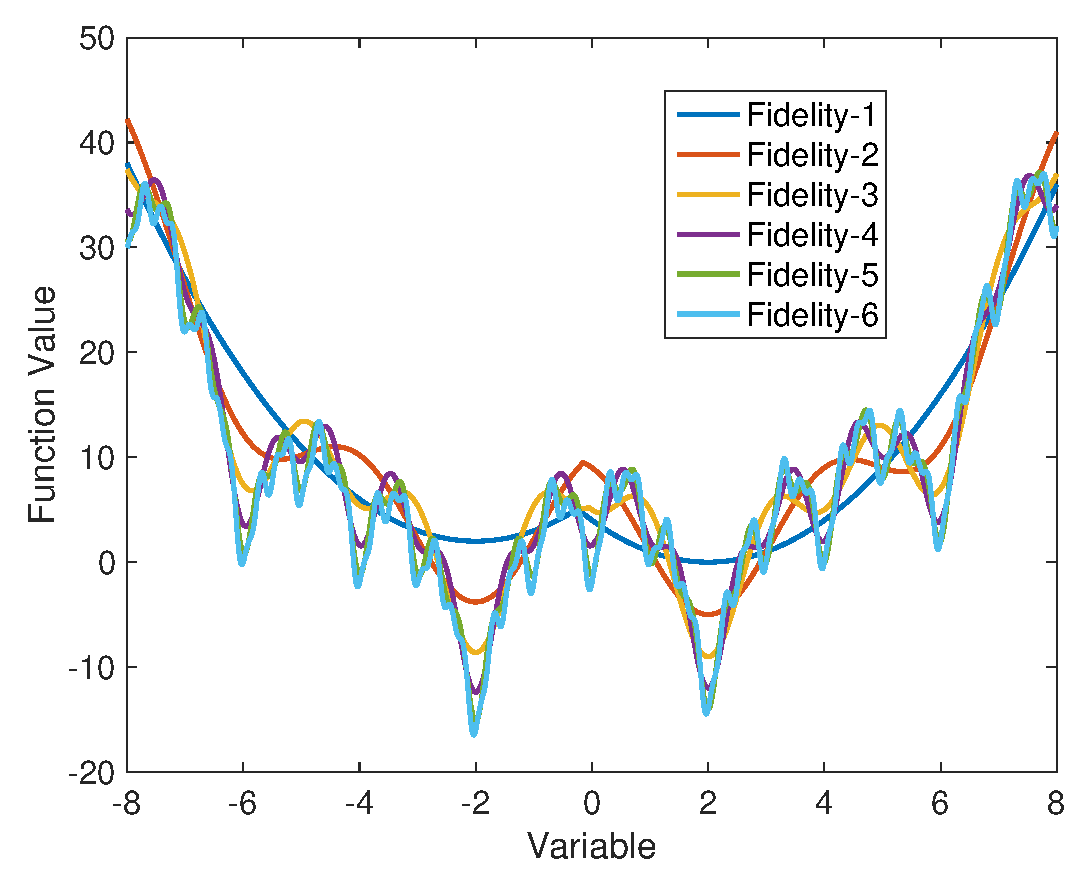
\includegraphics[scale=.4]{Figures/Figure1.eps}
		\caption{Test Function}
		\label{fig:test_fn2}
	\end{center}       
\end{figure}

\begin{table}[!htb]
	\caption{Mean squared error~(MSE) and the rank correlation coefficient (Kendall Tau) between the fidelities of the 1-dimensional artificial test function.}
	\label{table:mse_tau_test_fn2}
	\begin{center}
		\begin{tabular}{c|c|c}
			\hline
			&MSE&Kendall Tau\\
			\hline
			$f^1$ &35.3972 & 0.6380 \\
			$f^2$ &20.2299 & 0.6724\\
			$f^3$ &9.9857 & 0.7853\\
			$f^4$ &3.8126 & 0.8686\\
			$f^5$ &0.8242 & 0.9409\\
			$f^6$ &0.0000 & 1.0000\\
			\hline
		\end{tabular}
	\end{center}
\end{table}

The function can be extended to multiple dimensions by simply using the same function in each dimension, and adding up the values. For the two-dimensional version, the MSE and Kendall Tau values are reported in Table~\ref{table:mse_tau_2d}.

\begin{table}[!htb]
	\caption{Mean squared error~(MSE) and the rank correlation coefficient (Kendall Tau) between the fidelities of the 2-dimensional artificial test function.}
	\label{table:mse_tau_2d}
	\begin{center}
		\begin{tabular}{c|c|c}
			\hline
			&MSE&Kendall Tau\\
			\hline
			$f^1$ &78.8834 & 0.6694 \\
			$f^2$ &45.7713 & 0.7500\\
			$f^3$ &22.9244 & 0.8292\\
			$f^4$ &8.9905 & 0.8962\\
			$f^5$ &1.9883 & 0.9528\\
			$f^6$ &0.0000 & 1.0000\\
			\hline
		\end{tabular}
	\end{center}
\end{table}


\subsection{Toysub Benchmark Problem}
As a complement to the artificially designed one-dimensional benchmark function, the toysub benchmark problem is designed to be more similar to a real-world problem.
The task is to design a toy submarine (Fig.~\ref{fig:dallas_photo}) with the goal to minimize the drag, while still obeying all volume constraints. The problem involves eight variables defining the geometry of the submarine as shown in Fig.~\ref{fig:toysub_param_illum}. The design variables are: the position of the internal components along the $Z$-axis i.e. the position of the controller ($Z_C$), position of the propeller unit for pitch ($Z_V$) and yaw ($Z_L$) movements, position of the battery compartment ($Z_B$), smaller diameter ($d_t$) and length ($l_t$) of the tail and shape variation coefficient ($n_n$) and length ($l_n$) of the nose. The bounds of the variables are presented in Equation~\ref{eq:formulation_toysub}. The drag is estimated using ANSYS FLUENT 13.0.

The overall problem can be formulated as follows:
\begin{equation}
\begin{array}[p]{l}
\text{Minimize:}f\left(1\right) = D \\
\text{Variable bounds:}
\\
0 \le Z_C \le 300~mm;~~0 \le Z_V \le 300~mm
\\
0 \le Z_B \le 300~mm;~~0 \le Z_L \le 300~mm
\\
35 \le d_t \le 50~mm;~~80 \le l_t \le 150~mm
\\
1.5 \le n_n \le 3;~~45 \le l_n \le 100~mm
\label{eq:formulation_toysub}
\end{array}
\end{equation}

However, testing each solution using the CFD solver would make solving the problem too time consuming to be a sensible benchmark. Also, only researchers with access to the ANSYS FLUENT 13.0 software would be able to replicate results or compare their algorithms. Since the body is axisymmetric, a quarter model of the bare hull can be used to reduce the CFD analysis costs, but it would still be too slow to be practical.
To solve this predicament, we have generated 284 designs using Latin Hypercube Sampling and estimated their drag using ANSYS FLUENT 13.0. The velocity at the inlet was set to $0.5$~m/s while that at the outlet was set to zero. We recorded the drag values for these designs after 5, 10, 25, 50, 75 and 100 iterations resulting in 6 different fidelity levels with computational cost of 5, 10, 25, 50, 75 and 100 units, respectively. 
This data was then "expanded" to the full range of the search space by learning six Gaussian Process models based on the 284 design points, one for each fidelity level. These six Gaussian Process models hopefully correspond closely to the landscapes of the real CFD solver, but are much faster to evaluate and thus constitute a suitable benchmark problem. 

The mean squared error and the correlation coefficient (Kendall Tau) between the various fidelity levels and the highest fidelity level based on 1000 uniformly distributed random designs are presented in Table~\ref{table:mse_tau_toysub}. Again, Kendall Tau is increasing with increasing fidelity level, while mean squared error is generally decreasing (although not monotonically). 

\begin{figure}[!htb]
	\begin{center}
		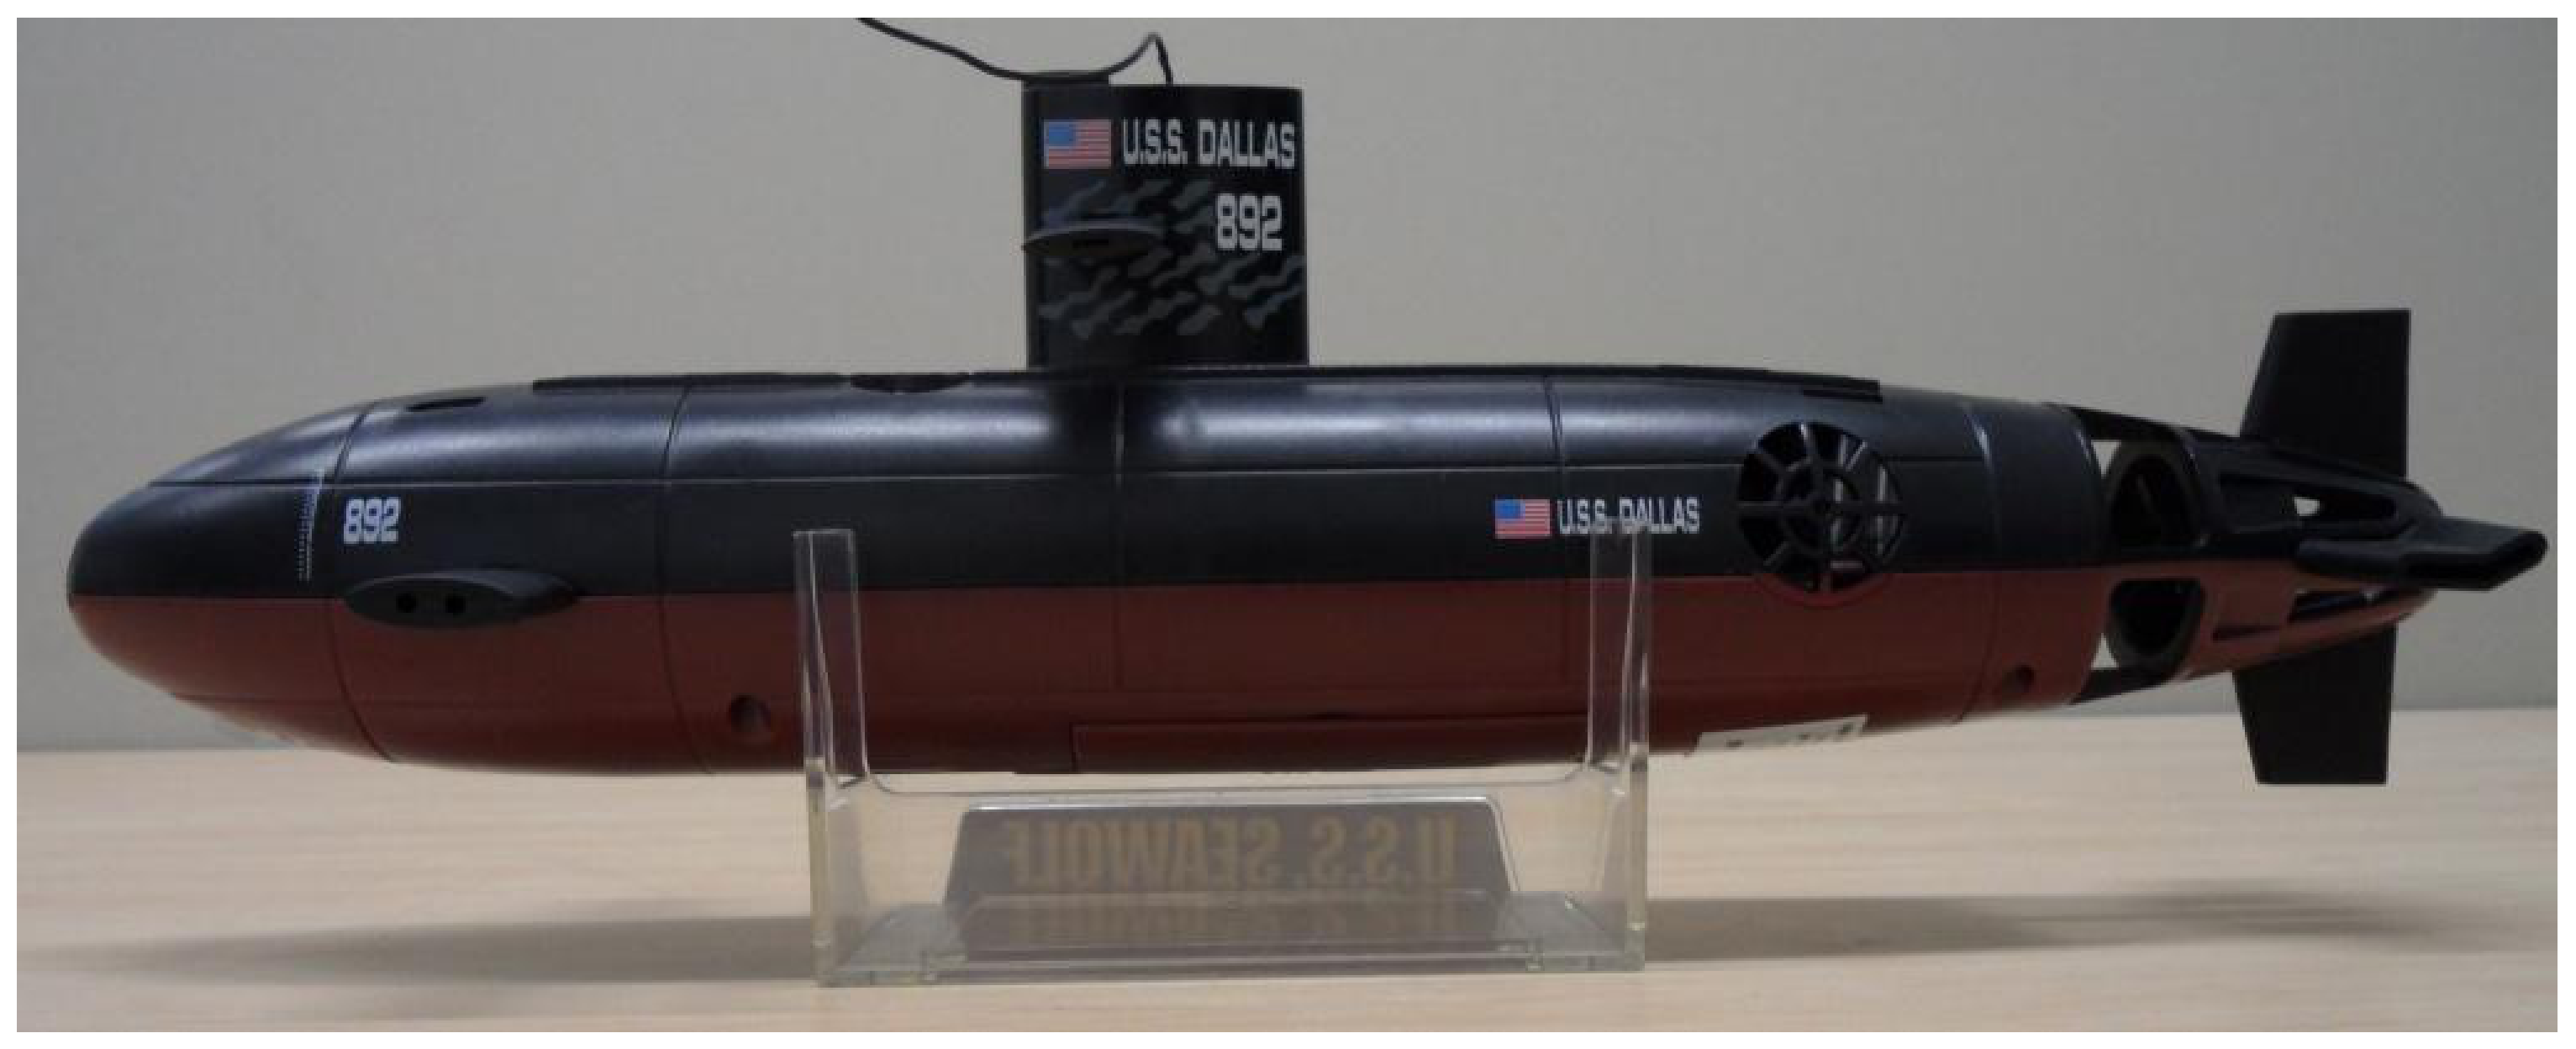
\includegraphics[width=3.55 in]{Figures/Figure2.eps}
		\caption{USS Dallas RC toy submarine}
		\label{fig:dallas_photo}
	\end{center}       
\end{figure}

\begin{table}[!htb]\scriptsize
	\caption{Performance criteria of the USS Dallas RC toy submarine}
	\label{table:performance_criteria_toysub}
	\centering
	\begin{tabular}{p{2.0in} l}
		\hline
		Vehicle particulars & USS Dallas RC\\
		\hline
		Nose length & 45~mm \\
		Parallel middle body length & 210~mm\\
		Tail length & 95~mm\\
		Length overall & 350~mm\\
		Maximum diameter & 60~mm\\
		Length to diameter ratio & 5.8\\
		Wetted surface area & 0.082385~m{$^2$}\\
		Displacement volume & 0.000437~m{$^3$}\\
		Mass of the displaced water & 437~g\\
		Total mass of the vehicle & 430~g\\
		X-coordinate of CG & -0.981462~mm\\
		Y-coordinate of CG & -0.210313~mm\\
		Z-coordinate of CG & 167.083~mm\\
		X-coordinate of CB & 0\\
		Y-coordinate of CB & 0\\
		Z-coordinate of CB & 163.375~mm\\
		Nominal speed & 0.5~m/s\\
		Drag & 0.0671897~N\\
		\hline
	\end{tabular}
\end{table}



\begin{figure}[!ht]
	\begin{center}
		\includegraphics[width=0.45\textwidth]{Figures/Figure3.eps}
		\caption{Design variables}
		\label{fig:toysub_param_illum}
	\end{center}       
\end{figure}





\begin{table}[!htb]
	\caption{Mean squared error~(MSE) and the rank correlation coefficient (Kendall Tau) between the functions}
	\label{table:mse_tau_toysub}
	\begin{center}
		\begin{tabular}{c|c|c}
			\hline
			&MSE&Kendall Tau\\
			\hline
			$y^1$ & 0.0203 & 0.7735\\
			$y^2$ & 0.0011 & 0.8712\\
			$y^3$ & 0.0017 & 0.8936\\
			$y^4$ & 0.0000 & 0.9791\\
			$y^5$ & 0.0000 & 0.9899\\
			$y^6$ & 0.0000 & 1.0000\\
			\hline
		\end{tabular}
	\end{center}
\end{table}


\section{Empirical Evaluation\label{sec:results}}
\subsection{Parameter Settings}
%To solve this problem, one can opt to use any single fidelity analysis within an optimization scheme and evaluate the final population using the highest fidelity estimate. The results of optimization using all possible single fidelity analysis is presented below. 

As the underlying optimization algorithm, we uased a real coded evolutionary algorithm with simulated binary crossover and polynomial mutation \cite{Deb01}. The probability of crossover is set to 1 with a mutation probability of 0.1 for the simple test function and 0.125 for the Toysub problem. The distribution indices of crossover ($\eta_c$) and mutation($\eta_m$) are set to $20$ and $30$ respectively, independent of the optimization problem. 
Population size is 20 for the simple one-dimensional function, and 48 for the more complicated Toysub problem.
The total evaluation budget was limited to $2000$ units for the simple test function and 100,000 units for the Toysub problem. 

The initial probability threshold for MFEA is $\delta=0.05$ unless stated otherwise, and linearly decreased to zero over the course of the run to ensure that no selection errors are made at the late stages of the optimization run.


\subsection{Performance Measure and Benchmarks}

To evaluate the performance of our proposed MFEA algorithm, we compare it with the following alternative approaches:
\begin{enumerate}
	\item {\bf Fidelity-6:} Evolutionary algorithm where every solution is evaluated with the highest fidelity model. 
	\item {\bf Fidelity-1:} Evolutionary algorithm where every solution is evaluated with the lowest fidelity model.
	\item {\bf Average:} In principle, one could also compare with the performance using any other fixed fidelity model. However, for a real world problem, it would not be clear which fidelity level would result in the best solution quality. To reflect this fact, we assume the user might pick a fidelity level at random. Then, the expected performance would just be the average of the expected performances of each fidelity level.
	\item {\bf Progressive:} Some people have suggested starting with a low fidelity model and then moving to a higher fidelity model over the course of the optimization. We have implemented this by dividing up the computational budget into equal parts, and using the same computational budget on each fidelity level.
\end{enumerate}

We are interested in the highest fidelity performance of the solution returned by the algorithm. Independent of the algorithm variant, the final generation is evaluated to the highest fidelity to make sure that the best solution in the population is recognized and accounted for. 

Different algorithms may have advantages at different stages of the run. For example, an algorithm using only the lowest fidelity can be expected to do well if the computational budget is very small, as it can still perform a few generations albeit with a crude fitness approximation. On the other hand, if the computational budget is very large, then we can assume that an algorithm only using the highest fidelity model will yield the best result. Thus it is important to look at the convergence plots of the algorithm. The convergence plots we use show the highest fidelity performance of the solution that would be returned at a particular point in time, where time includes the high fidelity evaluation of the final population. 

The generation of the convergence plot is best explained by an example. Let us consider a run on the simple function with fixed fidelity 2. The initial population requires 40 cost units to evaluate at fidelity level 2. If we were to stop here, this population would be fully evaluated, which requires another 80 cost units (four additional fidelity levels for 20 solutions). So, our first entry on the convergence plot would be the best solution according to fidelity level 6, with a cost of 120 units. The algorithm continues from the level 2 evaluation, generates 20 children and selects the next population. On the convergence plot, we then plot the best solution based on fidelity level 6 with a cost of 160 units (40 for evaluating the initial population, 40 for evaluating the children, and 80 to bring all selected individuals to fidelity level 6, etc.).

All results reported are based on the average over 100 independent runs for the simple test function, and 30 independent runs for the Toysub problem.

\subsection{Results on the Simple Test Function}

Fig.~\ref{fig:simple} shows the convergence plot for various different methods on the simple artificial test problem. As expected, the EA with fidelity 1 converges quicker than the other algorithms, but to a rather poor solution. The EA using fidelity 6 is able to find a much better solution eventually, but is the slowest to converge. Somewhat surprising is the poor performance of the progressive EA. It seems it is quickly misguided into the wrong area of the search space by fidelity 1, and then not able to recover by the time it switches to a higher fidelity. Our MFEA works quite well over the entire run.

The observations are reinforced also by looking at Tables~\ref{tab:simpleFinal} and \ref{tab:simpleArea}, which show the algorithm performance after a computational budget of 2000 units and as average over the runtime, respectively. While the Fidelity-6 approach yields the best performance at the end of the run, it is only marginally better than our MFEA and the difference is statistically not significant. In terms of average performance over the run, MFEA statistically outperforms all other approaches in the table. 

Similar observations hold for the 2D version of this test function, see Fig.~\ref{fig:test2DForcing}.

\begin{figure}[!htb]
	\centering
	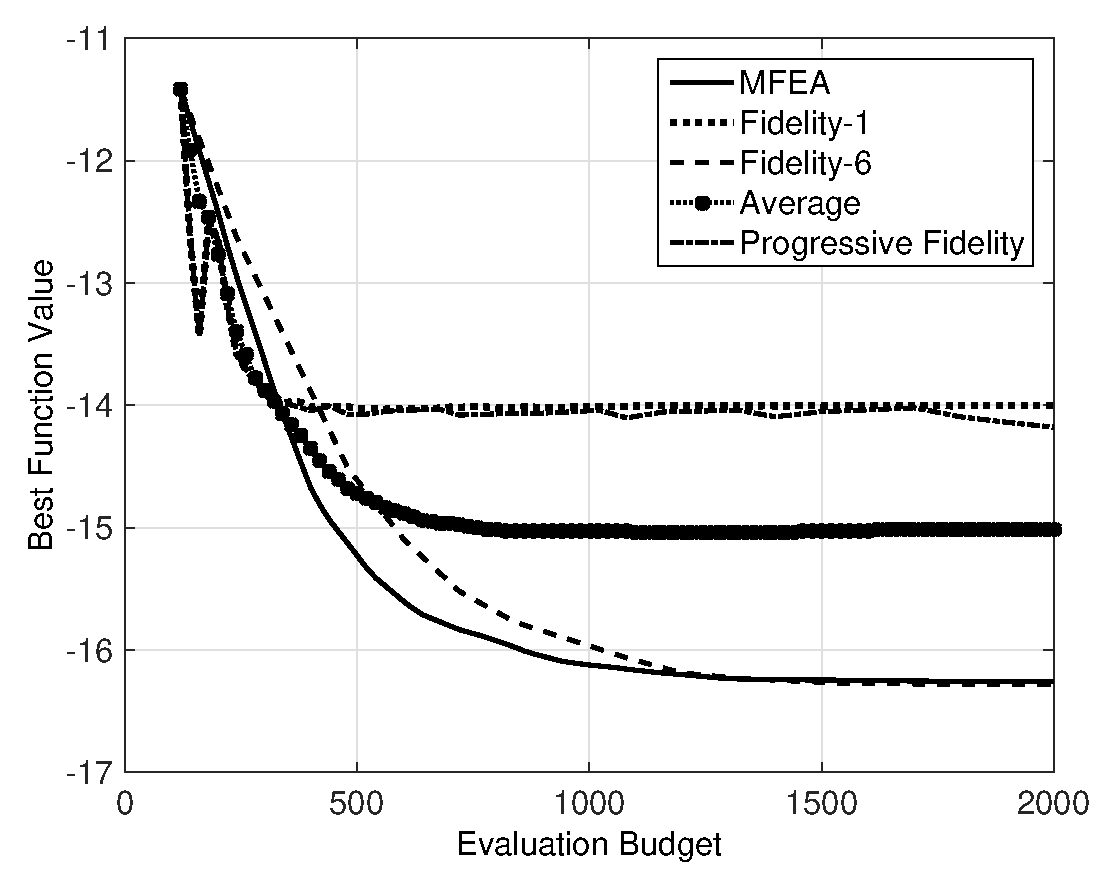
\includegraphics[width=\linewidth]{Figures/Figure4.eps}
	\caption{Convergence plot for various approaches on the simple 1D test function}
	\label{fig:simple}
\end{figure} 

\begin{figure}[!htb]
	\centering
	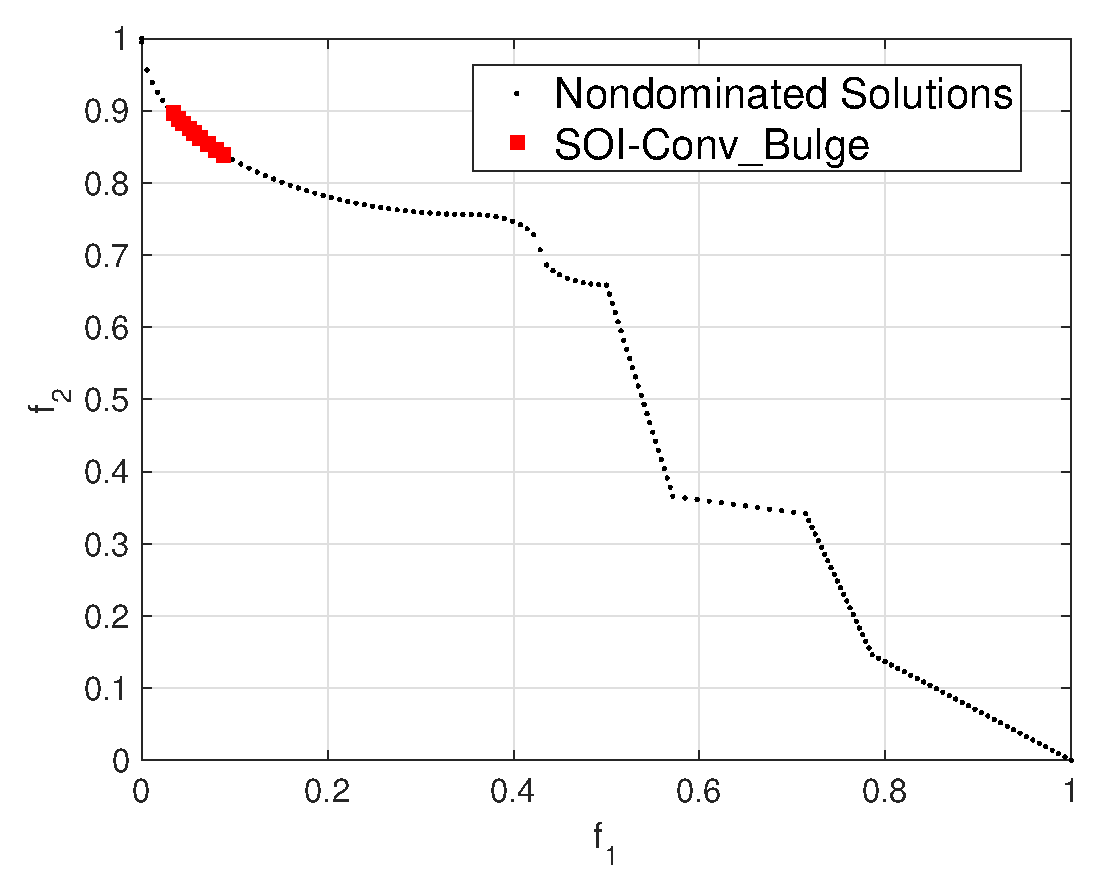
\includegraphics[width=\linewidth]{Figures/Figure5.eps}
	\caption{Convergence plot for various approaches on the simple 2D test function}
	\label{fig:test2DForcing}
\end{figure}



\begin{table}[!ht]\footnotesize
	\centering
	\caption{Performance obtained at end of run for simple test function.}
	\label{tab:simpleFinal}
	\begin{tabular}{l|l|l|l|l|l}
		\hline
		\textbf{Test function}        & \textbf{Best} & \textbf{Mean} & \textbf{Median} & \textbf{Worst} & \textbf{Std Err} \\ \hline
		\textbf{MFEA}           & -16.475       & -16.259       & -16.469         & -14.462        & 0.057              \\ 
		\textbf{Fidelity-1}           & -14.071       & -14.002       & -14.000         & -13.965        & 0.002              \\ 
		\textbf{Fidelity-2}           & -14.346       & -13.997       & -14.000         & -13.609        & 0.008              \\ 
		\textbf{Fidelity-3}           & -16.398       & -14.150       & -14.005         & -13.577        & 0.054              \\ 
		\textbf{Fidelity-4}           & -16.371       & -15.851       & -16.001         & -13.933        & 0.060              \\ 
		\textbf{Fidelity-5}           & -16.475       & -15.786       & -16.000         & -13.534        & 0.067              \\ 
		\textbf{Fidelity-6}           & -16.475       & -16.286       & -16.469         & -14.375        & 0.055              \\ 
		\textbf{Progr.\ Fidelity} & -14.475       & -14.194       & -14.213         & -13.679        & 0.021              \\ \hline
	\end{tabular}
\end{table}

\begin{table}[!ht]\footnotesize
	\centering
	\caption{Average performance over the run on the simple test function.}
	\label{tab:simpleArea}
	\begin{tabular}{l|l|l|l|l|l}
		\hline
		\textbf{Test function}        & \textbf{Best} & \textbf{Mean} & \textbf{Median} & \textbf{Worst} & \textbf{Std Err} \\ \hline
		\textbf{MFEA}           & -16.475       & -15.592       & -15.731         & -13.027        & 0.070        \\ 
		\textbf{Fidelity-1}           & -14.149       & -13.922       & -13.973         & -13.434        & 0.016        \\ 
		\textbf{Fidelity-2}           & -14.557       & -13.962       & -14.024         & -12.891        & 0.029        \\ 
		\textbf{Fidelity-3}           & -16.035       & -14.254       & -14.217         & -12.989        & 0.055        \\ 
		\textbf{Fidelity-4}           & -16.348       & -15.490       & -15.667         & -13.549        & 0.064        \\ 
		\textbf{Fidelity-5}           & -16.398       & -15.355       & -15.522         & -13.487        & 0.073        \\ 
		\textbf{Fidelity-6}           & -16.475       & -15.402       & -15.650         & -10.308        & 0.094        \\ 
		\textbf{Progr.\ Fidelity} & -14.339       & -13.971       & -14.024         & -13.208        & 0.020        \\ \hline
	\end{tabular}
\end{table}

%\subsubsection{Probability of reversal and misclassification error}

Fig.~\ref{fig:prconvergence} examines the influence of the initial probability of reversal threshold $\delta$. As can be seen, the performance is quite robust to this parameter.

\begin{figure}[!htb]
	\centering
	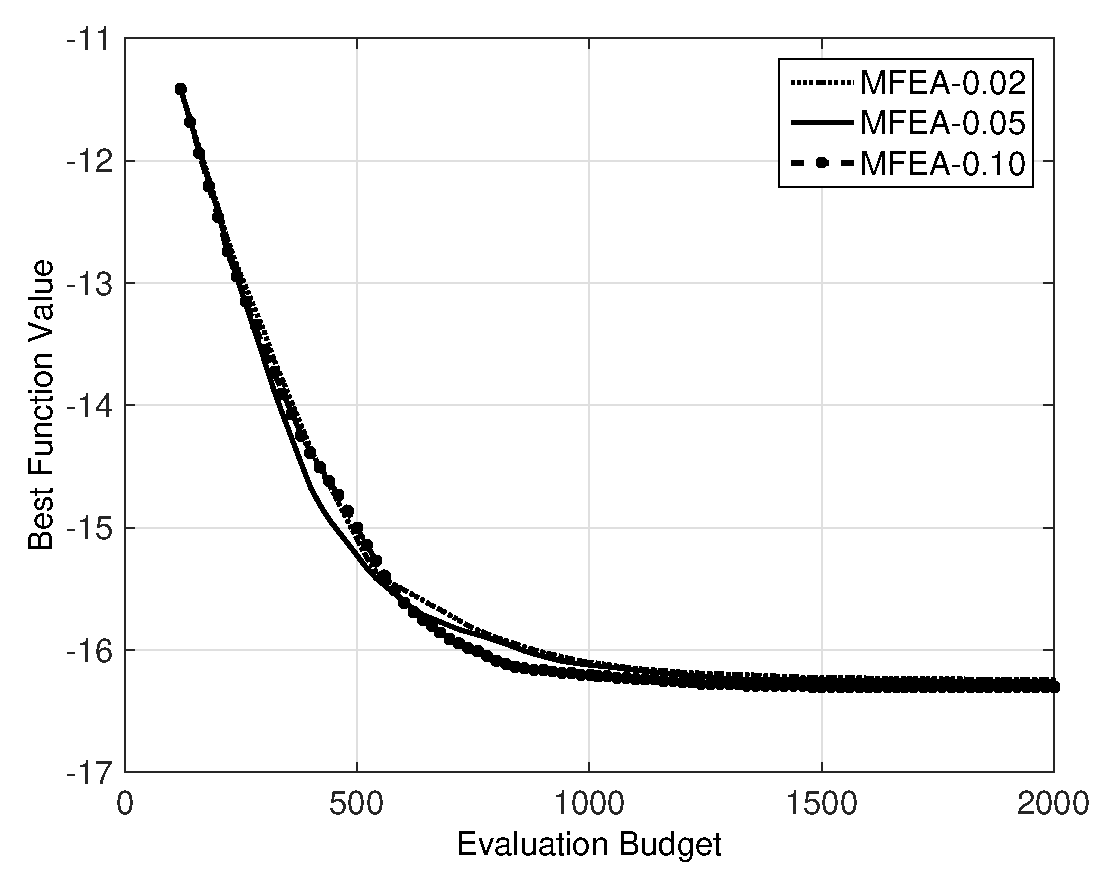
\includegraphics[width=\linewidth]{Figures/Figure6.eps}
	\caption{Convergence plot for various probability of reversal thresholds $\delta$ on the simple test function}
	\label{fig:prconvergence}
\end{figure} 

\begin{figure}[!htb]
	\centering
	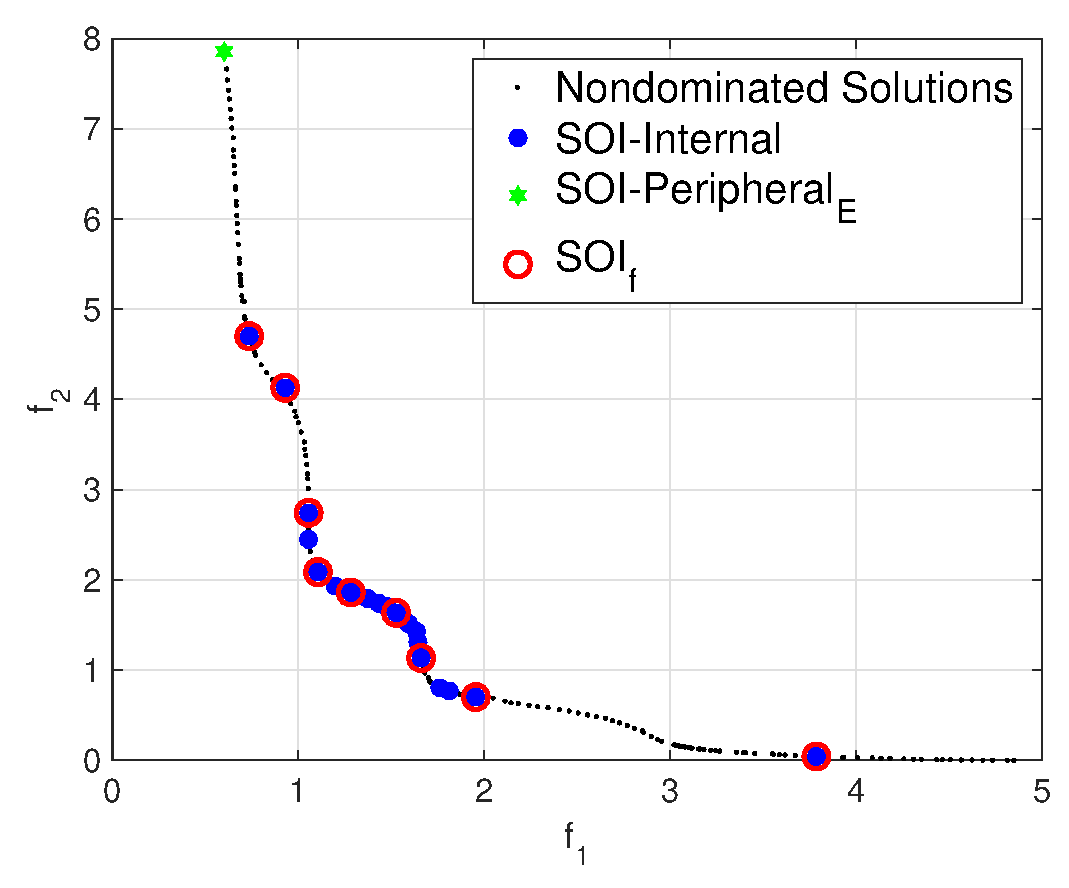
\includegraphics[width=\linewidth]{Figures/Figure7.eps}
	\caption{Percentage of misclassified individuals over the run, for different levels of reversal threshold $\delta$}
	\label{fig:simpleMisclassify}
\end{figure} 


To gain a better understanding of the workings of the proposed algorithm, we investigated various other aspects on the 1D artificial test function. 
Fig.~\ref{fig:simpleMisclassify} shows the misclassification percentage over time, i.e., the percentage of solutions that have been unjustly (according to highest fidelity level) carried forward from one generation to the next. If this is zero, then we know survival selection works perfectly as if all individuals would have been evaluated at the highest fidelity level. As can be seen, for this simple test problem there is a small misclassification percentage at the beginning of the run, at least for  $\delta=0.05$ and $\delta=0.1$. It then quickly goes to zero, and there are no more errors in selection for the remainder of the run.

Fig.~\ref{fig:LRmodelInit} and \ref{fig:LRmodelFinal} show the probability of reversal as learned by the algorithm (one LR-model learned for each fidelity) for the initial and final generation, respectively. As would be expected, since the lower fidelity models are less reliable, for a given fitness difference $\Delta$ the predicted probability of reversal is generally higher (except for LR-models 4 and 5 which are very similar). Also, we see that the predicted probability of reversal reduces over the course of the run, probably because the algorithm zooms into a region around the optimum, and in this local region the correlation between the models is higher than over the entire search space.

\begin{figure}[!htb]
	\centering
	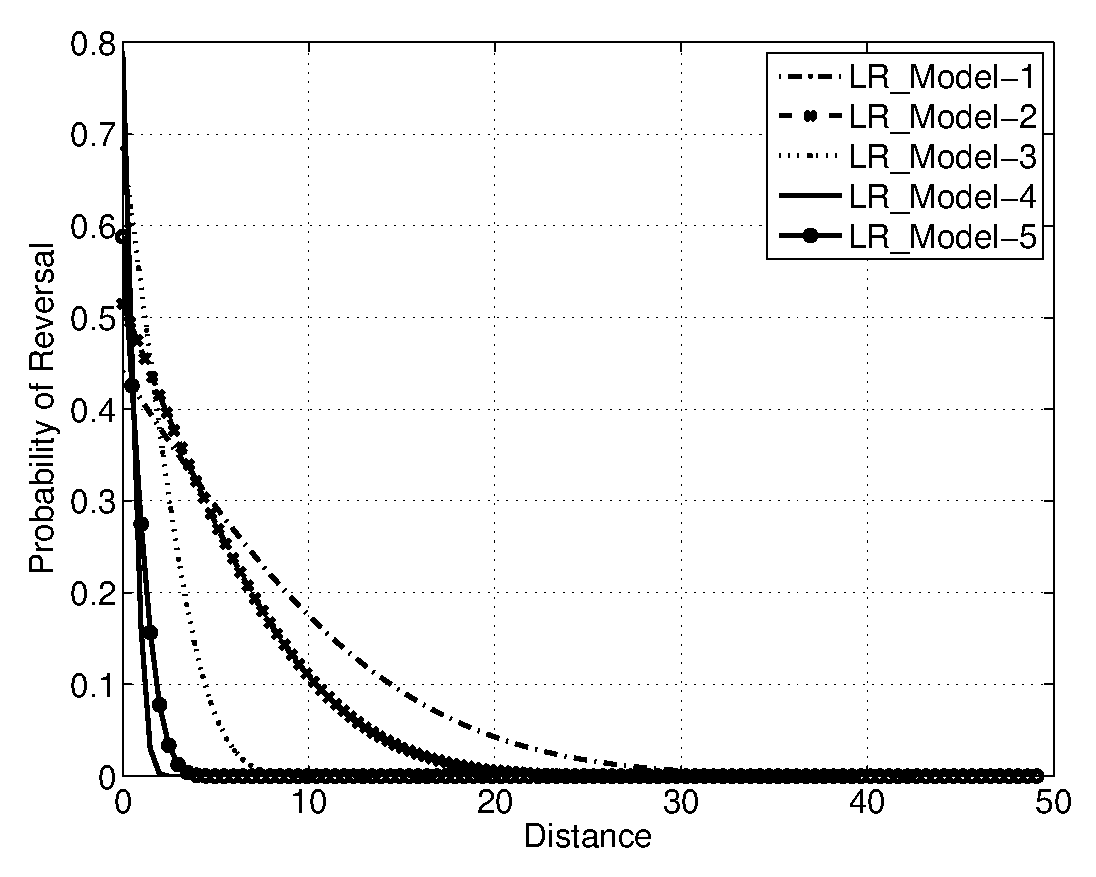
\includegraphics[width=\linewidth]{Figures/Figure8.eps}
	\caption{Learned model of probability of reversal just after initial population has been generated, for fidelity levels~1-5.}
	\label{fig:LRmodelInit}
\end{figure} 

\begin{figure}[!htb]
	\centering
	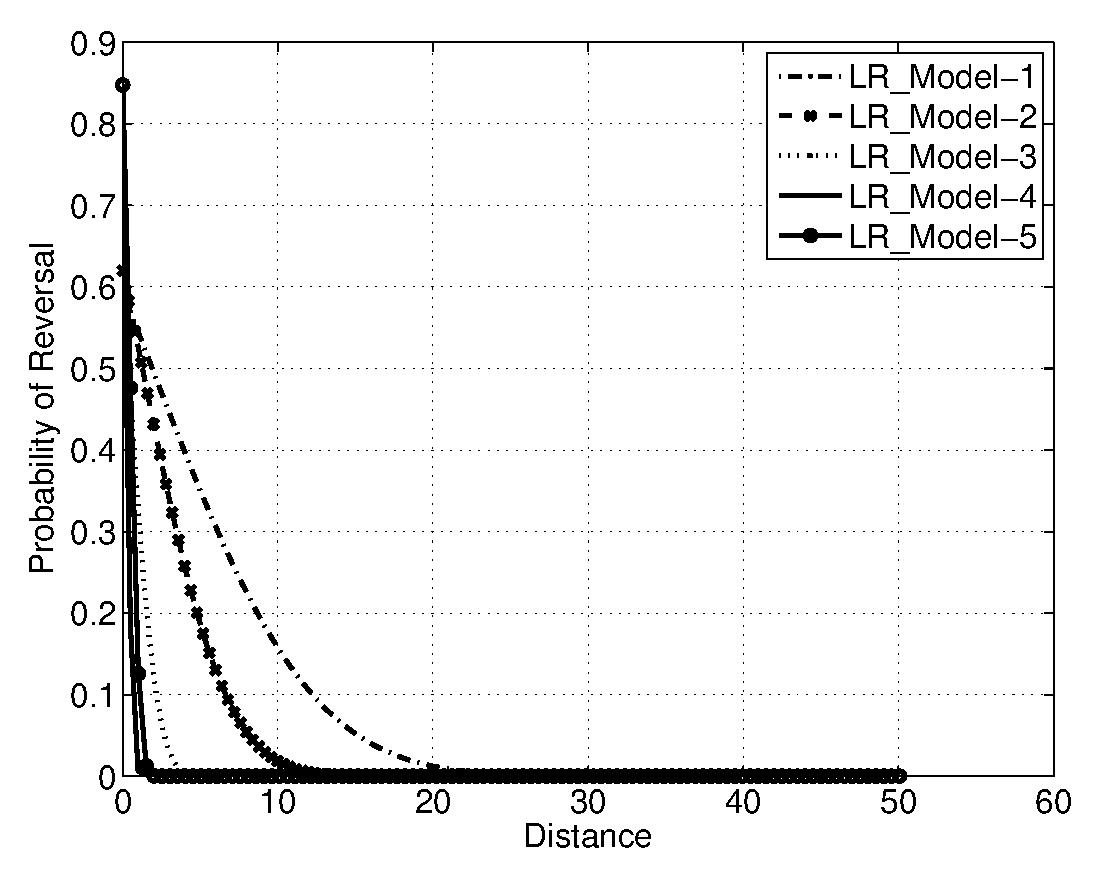
\includegraphics[width=\linewidth]{Figures/Figure9.eps}
	\caption{Learned model of probability of reversal at the end of an optimization run, for fidelity levels~1-5.}
	\label{fig:LRmodelFinal}
\end{figure} 

In our tests so far, we have assumed there are six levels of fidelity. However, a simulation run may be interrupted at many more possible stopping points, and each could be regarded as a fidelity level. There is a fundamental trade-off: More fidelity levels should allow our method to make better choices (albeit with diminishing returns, i.e., the difference between using 2 and 4 fidelity levels may be significant, whereas the difference between using 102 and 104 fidelity levels is probably marginal), but increases the training effort as we need to learn and update the probability of reversal for every fidelity level. To better understand the impact of the number of fidelity levels, Fig.~\ref{fig:testfidForcing} compares the convergence of MFEA that has access to all six fidelity levels with an MFEA that is only allowed to use fidelity levels~1 and 6. As expected, the larger number of fidelity levels leads to a slightly faster convergence.

\begin{figure}[!htb]
	\centering
	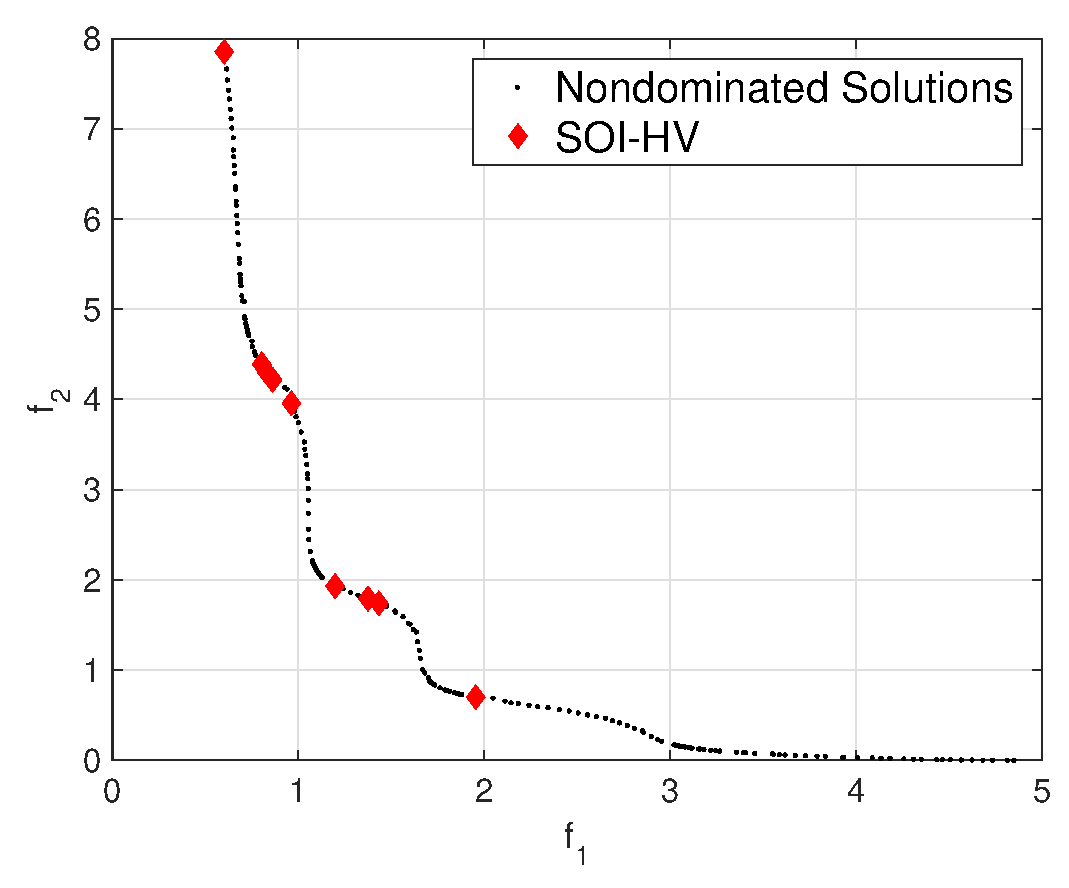
\includegraphics[width=\linewidth]{Figures/Figure10.eps}
	\caption{Comparison of convergence with different number of fidelity levels in forced condition for simple test function}
	\label{fig:testfidForcing}
\end{figure}

%\subsubsection{Forcing}
Finally, we wanted to understand the benefit of forcing at least one individual to be evaluated at the highest fidelity level in each generation. As Fig.~\ref{fig:simpleForcing} shows, in this example the effect of forcing on convergence seems marginal, with perhaps a small advantage in the early phases of the run.

\begin{figure}[!htb]
	\centering
	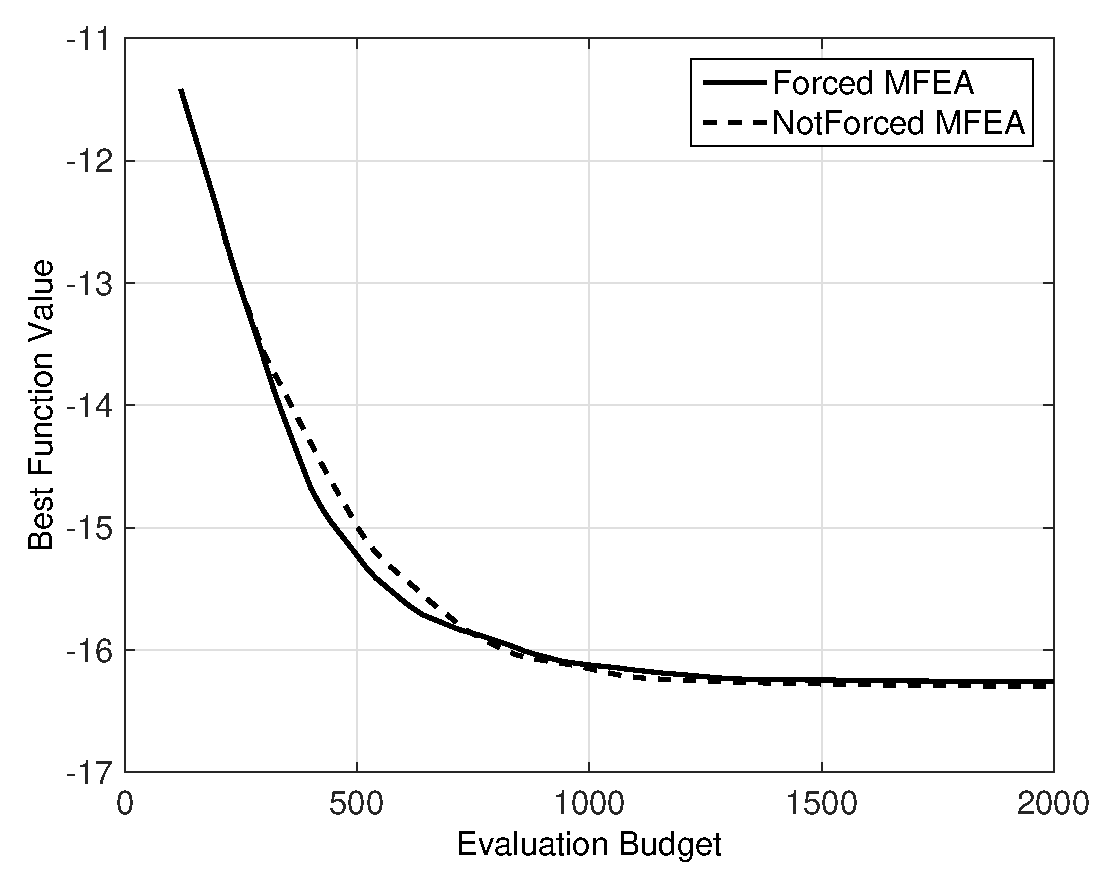
\includegraphics[width=\linewidth]{Figures/Figure11.eps}
	\caption{Convergence plot for MFEA with and without forcing on the simple test function}
	\label{fig:simpleForcing}
\end{figure} 

\subsection{Results on the Toysub Problem}

In addition to the single variable test function, in this section, we observe the performance on the close-to-real-world toy submarine design problem involving eight variables. Again, we first look at the convergence plot of various different approaches (Fig.~\ref{fig:toysub}). As for the simple test function, Fidelity-1 and the approach using progressive fidelity converge much quicker than the other approaches initially, but then get stuck in a local optimum. Fidelity-6 converges more slowly and finds a better solution, however this time not as good as our MFEA. This can probably be attributed to the fact that the computational budget of 100,000 was not sufficient to allow Fidelity-6 to converge. Our MFEA converges relatively quickly, and finds a very good solution within the given computational budget. In particular, MFEA only required about 40,000 computational units to reach the same solution quality that the high fidelity approach (Fidelity-6) has reached after a computational budget of 100,000 units, thus effectively saving 60\% of the computational cost.

\begin{figure}[!htb]
	\centering
	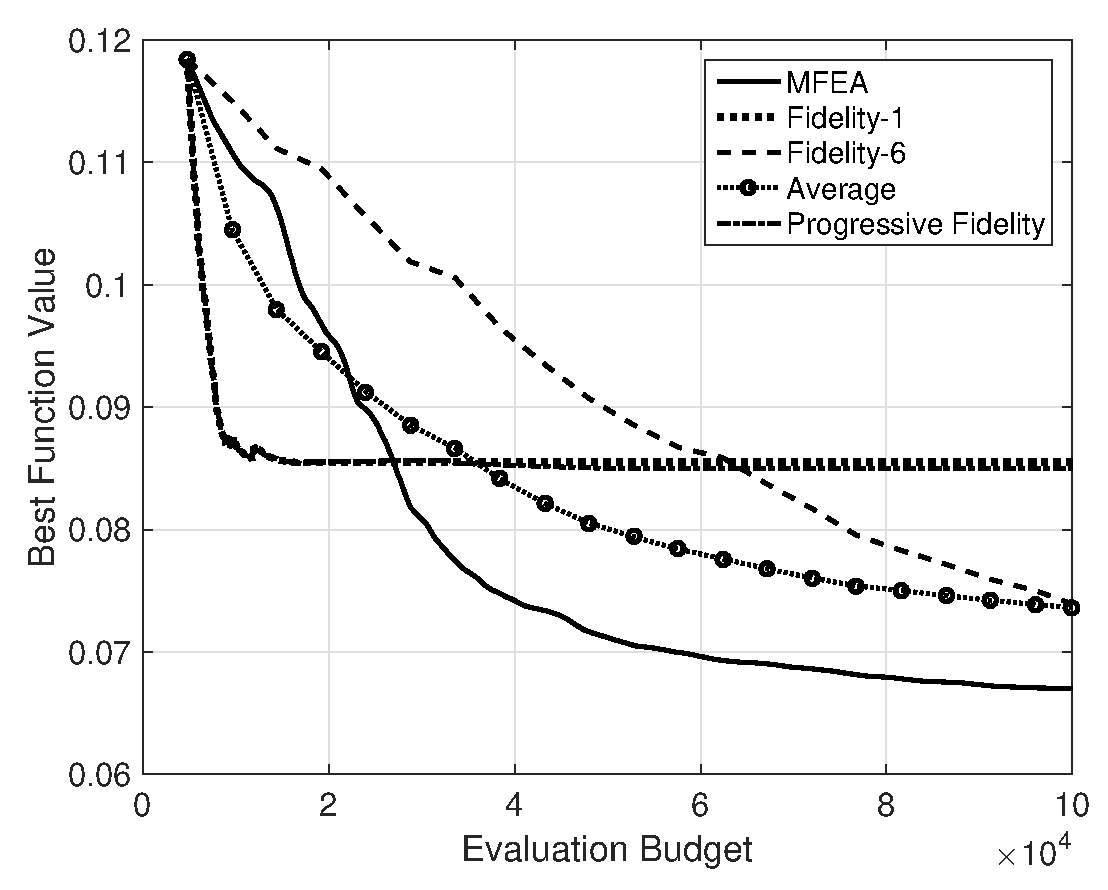
\includegraphics[width=\linewidth]{Figures/Figure12.eps}
	\caption{Convergence plot for various probability of reversal thresholds on the Toysub test problem.}
	\label{fig:toysub}
\end{figure} 

Looking at the results in Tables~\ref{tab:toysubBest} and \ref{tab:toysubArea}, this general impression is confirmed. MFEA significantly outperforms the progressive fidelity approach, and is significantly better than most single fidelity approaches as well. Fidelity-4 reaches a slightly better mean performance at the end than MFEA, however the difference is not statistically significant. In terms of average performance over the run, Fidelity-3 is slightly better, but again not statistically significant. Note that in a real world problem, one would not know which fidelity would yield best results with a given computational budget, so comparing the MFEA to the best of the single fidelity models is not a fair comparison.


Again, to gain a deeper understanding of the algorithm, we examine some additional aspects. When looking at the benefit of forcing (Figure~\ref{fig:toysubForcing}), this time there is a clearly visible benefit.

\begin{figure}[!htb]
	\centering
	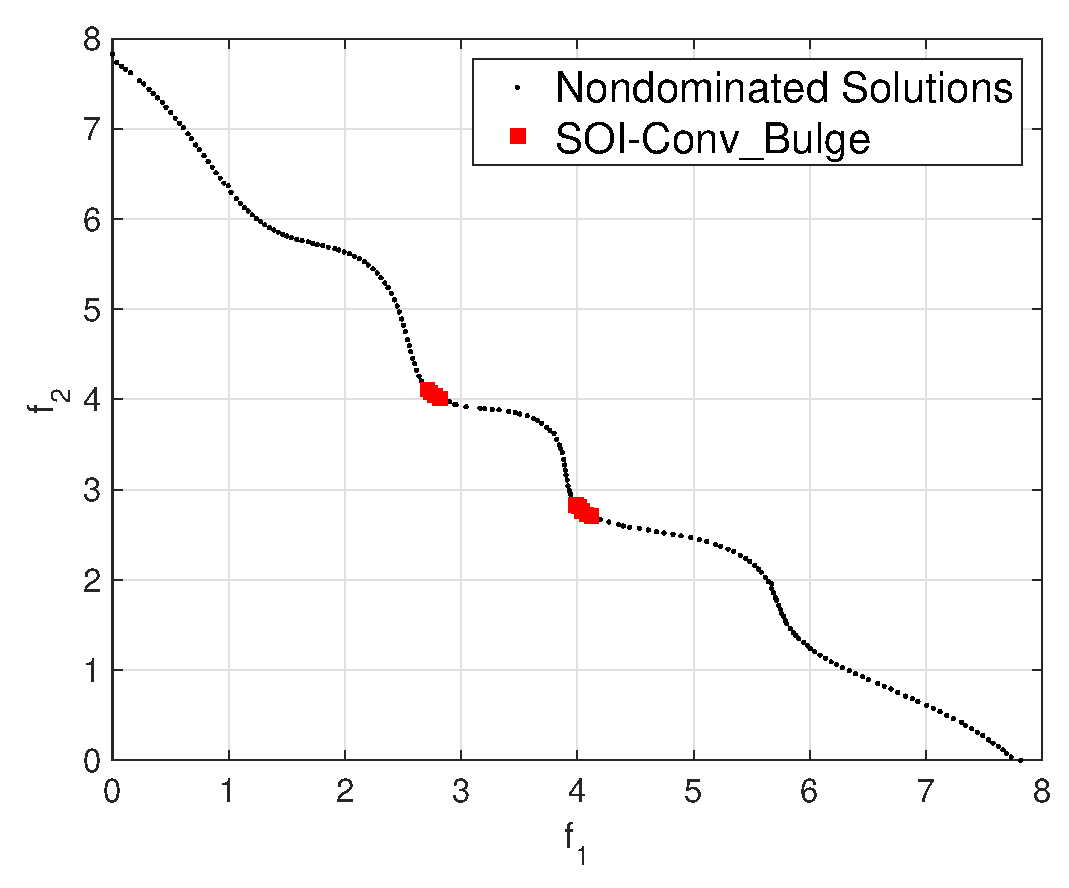
\includegraphics[width=\linewidth]{Figures/Figure13.eps}
	\caption{Convergence plot for MFEA with and without forcing on the Toysub test problem}
	\label{fig:toysubForcing}
\end{figure} 


\begin{table}[!ht]\footnotesize
	\centering
	\caption{Best function value: Toysub}
	\label{tab:toysubBest}
	\begin{tabular}{l|l|l|l|l|l}
		\hline
		\textbf{Toysub}               & \textbf{Best} & \textbf{Mean} & \textbf{Median} & \textbf{Worst} & \textbf{Std Err} \\ \hline
		\textbf{MFEA}           & 0.047         & 0.067         & 0.066           & 0.093          & 0.002              \\ 
		\textbf{Fidelity-1}           & 0.052         & 0.086         & 0.087           & 0.102          & 0.002              \\ 
		\textbf{Fidelity-2}           & 0.056         & 0.077         & 0.077           & 0.102          & 0.002              \\ 
		\textbf{Fidelity-3}           & 0.056         & 0.070         & 0.064           & 0.099          & 0.003              \\ 
		\textbf{Fidelity-4}           & 0.048         & 0.065         & 0.063           & 0.081          & 0.001              \\ 
		\textbf{Fidelity-5}           & 0.058         & 0.070         & 0.069           & 0.088          & 0.002              \\ 
		\textbf{Fidelity-6}           & 0.062         & 0.074         & 0.071           & 0.093          & 0.002              \\ 
		\textbf{Progr.\ Fidelity} & 0.052         & 0.085         & 0.086           & 0.102          & 0.002              \\ \hline
	\end{tabular}
\end{table}

\begin{table}[!ht]\footnotesize
	\centering
	\caption{Average performance over the run on the Toysub problem}
	\label{tab:toysubArea}
	\begin{tabular}{l|l|l|l|l|l}
		\hline
		\textbf{Toysub}               & \textbf{Best} & \textbf{Mean} & \textbf{Median} & \textbf{Worst} & \textbf{Std Err} \\ \hline
		\textbf{MFEA}           & 0.056         & 0.078         & 0.078           & 0.097          & 0.002        \\ 
		\textbf{Fidelity-1}           & 0.055         & 0.086         & 0.087           & 0.103          & 0.002        \\ 
		\textbf{Fidelity-2}           & 0.059         & 0.079         & 0.079           & 0.103          & 0.002        \\ 
		\textbf{Fidelity-3}           & 0.063         & 0.076         & 0.072           & 0.102          & 0.002        \\ 
		\textbf{Fidelity-4}           & 0.068         & 0.080         & 0.079           & 0.091          & 0.001        \\ 
		\textbf{Fidelity-5}           & 0.071         & 0.088         & 0.088           & 0.100          & 0.001        \\ 
		\textbf{Fidelity-6}           & 0.076         & 0.092         & 0.093           & 0.106          & 0.002        \\ 
		\textbf{Progr.\ Fidelity} & 0.055         & 0.086         & 0.087           & 0.103          & 0.002        \\ \hline
	\end{tabular}
\end{table}

%As can be seen, for this simple test problem the misclassification percentage is relatively low in the beginning, probably because the individuals are diverse and even the low fidelity models guide the search in the right direction. Then there is a phase of relatively high misclassification percentage, which we attribute to the fact that the search is narrowing down, and the learning algorithm needs some time to adjust. Finally, in the late stage of the algorithm, misclassification percentage is once more very small.

Fig.~\ref{fig:evals} shows the number of individuals that were evaluated at each fidelity level, for a typical run. Obviously, in each generation, the 48 children are all evaluated with fidelity 1. On the higher fidelity levels, it can be any subset of children plus a subset of the parents that have not yet been evaluated to this level. But we can see that, except for full evaluation of the initial population, the actual evaluations performed are clearly less than if all individuals would be evaluated in the highest fidelity. Also, there is a clear trend towards higher fidelity evaluations in the later stages of the run, which makes perfect sense as solutions to be compared become more similar, which makes a selection based on lower fidelity levels less reliable, and also because we use a linearly decreasing threshold for the probability of reversal.

\begin{figure}[!htb]
	\centering
	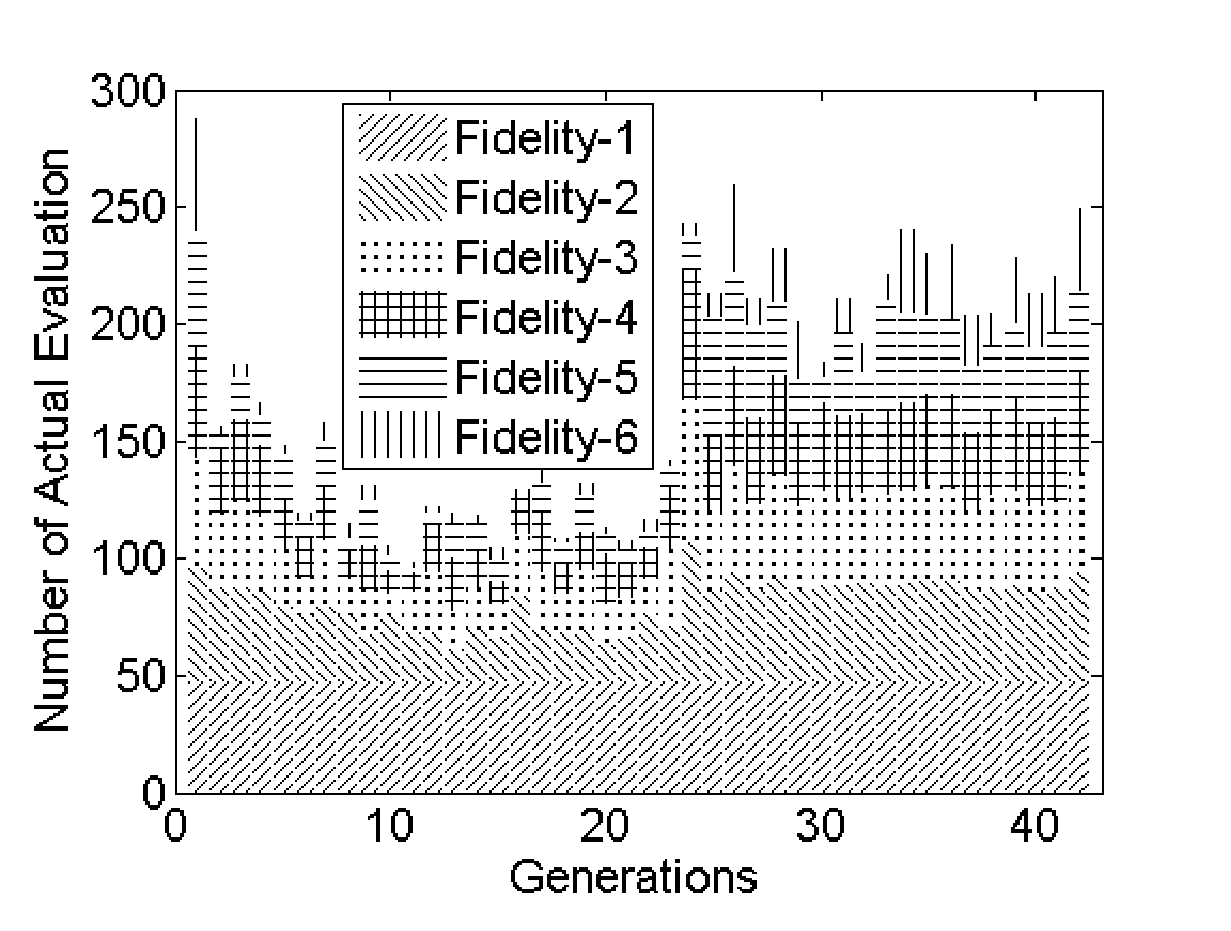
\includegraphics[width=1.06\linewidth]{Figures/Figure14.eps}
	\caption{Number of fitness evaluations performed at different fidelity levels, over the course of the run}
	\label{fig:evals}
\end{figure} 

Finally, we once again compare the convergence of MFEA that uses 6 fidelity levels to one that uses only fidelity levels~1 and 6. As can be seen in Fig.~\ref{fig:toysubfidForcing}, the larger number of fidelity levels is again beneficial, and the difference appears larger than for the artificial test problem in Fig.~\ref{fig:testfidForcing}.

\begin{figure}[!htb]
	\centering
	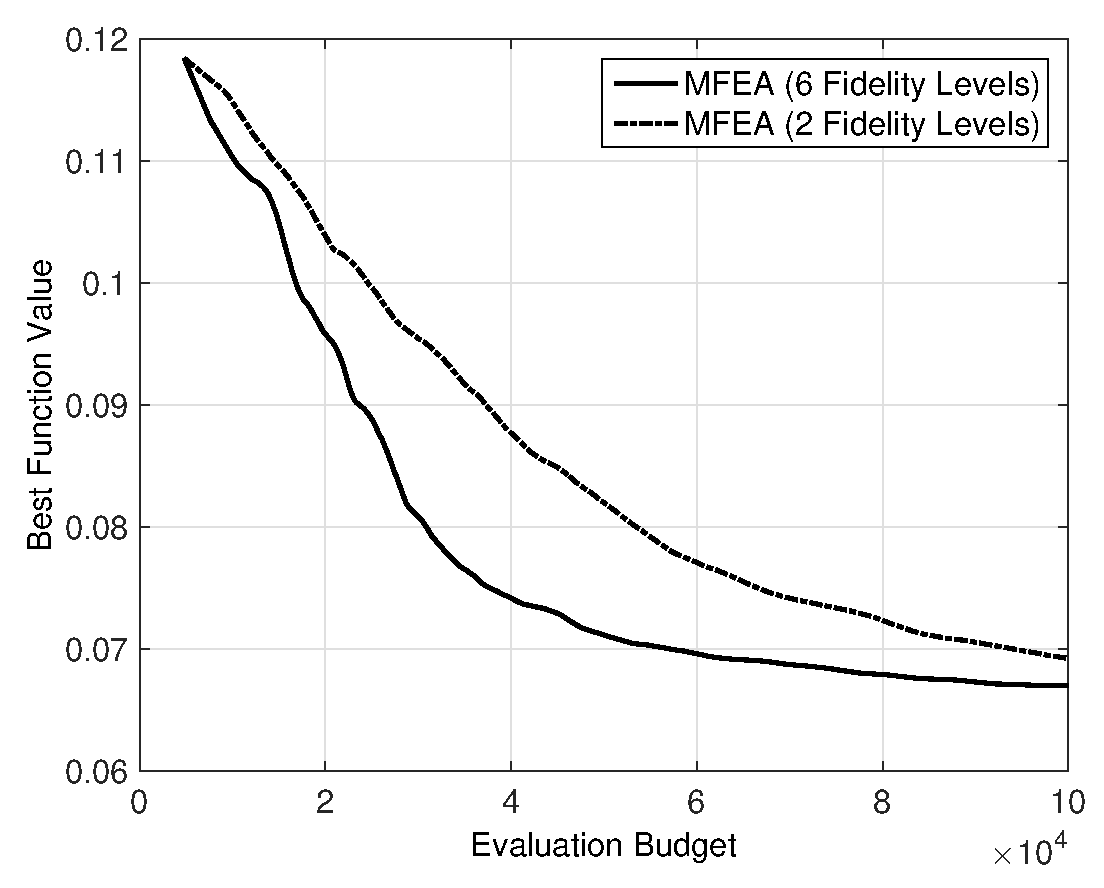
\includegraphics[width=\linewidth]{Figures/Figure15.eps}
	\caption{Comparison of convergence with different number of fidelity levels in forced condition for Toysub test problem}
	\label{fig:toysubfidForcing}
\end{figure}



\subsection{Additional Test Problems}
To better understand in what situations our algorithm might work well and whether it is able to adapt to different situations, we designed two additional test problems. In the first one, PF1, all the fidelities are identical and correspond to fidelity level~6 of our simple artificial test function. In such a case, clearly only using fidelity~1 is the best possible strategy, as higher fidelity levels do not provide more accurate information but only incur a higher computational cost. The opposite scenario is a problem where the different fidelities have nothing in common. We designed such a function PF2 by assigning each fidelity level independently a different function, sometimes shifted to make sure they don't happen to have the same optimum, see Table~\ref{tab:PF2} and Table~\ref{table:mse_tau_pf2} for the MSE and Kendall Tau correlation. For such a function, the best strategy should be to only use fidelity level~6, as lower fidelity levels do not provide useful information.



\begin{table}[!htb]
	\caption{Different fidelities of function PF2. The variable (x) range for all levels is set to [-8, 8].\label{tab:PF2}}
	\begin{center}
		\begin{tabular}{c|c}
			\hline
			Fidelity&Function\\
			\hline
			f1(x)& Ackley(x-0.8)\\
			f2(x)& Griewank(x-0.6)\\
			f3(x)&  Sphere(x)\\
			f4(x)&  -1$\times$Rastrigin(x-0.1)\\
			f5(x)&  Zakharov(x-0.4)\\
			f6(x)&  -1$\times$Levy(x-0.2)\\
			\hline
		\end{tabular}
	\end{center}
\end{table}


The results on these two problems are depicted in Fig.~\ref{fig:pf1} and \ref{fig:pf2}.
As expected, for PF1, using fidelity~1 only would perform best. Our MFEA is a bit slower in the beginning as it has to learn first that higher fidelity levels are not helpful, and the forcing mechanism forces the algorithm to fully evaluate at least one individual in every generation. Still, it is much faster than picking a fidelity level at random or using the highest fidelity only. For example, where the algorithm using fidelity~6 requires approx.\ 1500 function evaluations to converge, MFEA only requires a third, i.e., approx.\ 500 function evaluations.
Using a progressive fidelity level also works very well for this function, basically because it starts with fidelity~1 and has almost converged by the time it switches to the next higher fidelity level.

For PF2, clearly fidelity level 6 is required to allow any sensible optimization. Again, MFEA adapts to that scenario and performs almost as well as the algorithm with pre-set fidelity level~6. MFEA learns the correct fidelity level very quickly and, different from PF1, forcing is not causing unnecessary function evaluations. The algorithms with a pre-set lower fidelity level optimize the wrong function, and their performance actually deteriorates compared with the random initial population. 

From these experiments, we conclude that MFEA is very effective at learning the right fidelity level and thus should work well in a wide range of problem types.



\begin{figure}[!htb]
	\centering
	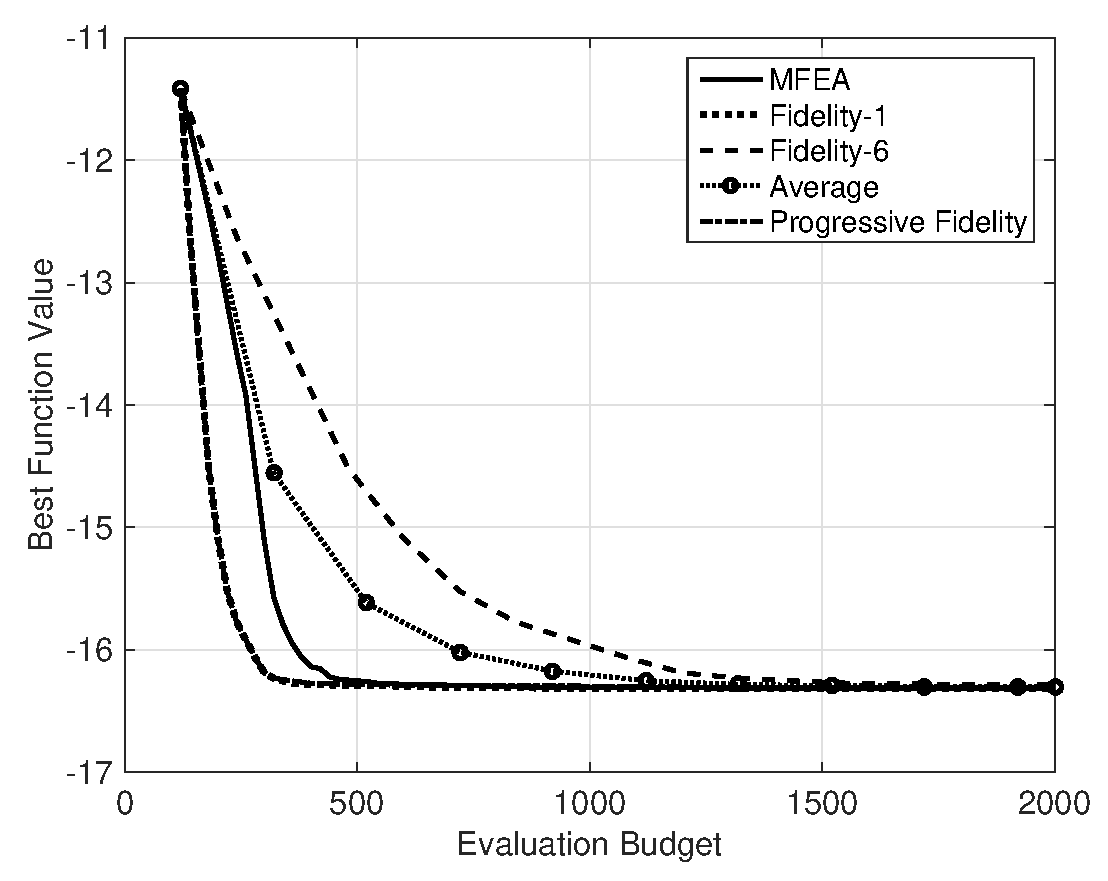
\includegraphics[width=\linewidth]{Figures/Figure16.eps}
	\caption{Convergence plot for various approaches on the PF1 test function.}
	\label{fig:pf1}
\end{figure} 

\begin{table}[!htb]
	\caption{Mean squared error~(MSE) and the rank correlation coefficient (Kendall Tau) between the functions in PF2.}
	\label{table:mse_tau_pf2}
	\begin{center}
		\begin{tabular}{c|c|c}
			\hline
			&MSE&Kendall Tau\\
			\hline
			$f^1$ &0.2441E+03 & -0.7124 \\
			$f^2$ &0.0177E+03 & 0.1047\\
			$f^3$ &1.0159E+03 & -0.6226\\
			$f^4$ &0.6857E+03 & 0.6402\\
			$f^5$ &16.2488E+03 & -0.7035\\
			$f^6$ &0.0000 & 1.0000\\
			\hline
		\end{tabular}
	\end{center}
\end{table}

\begin{figure}[!htb]
	\centering
	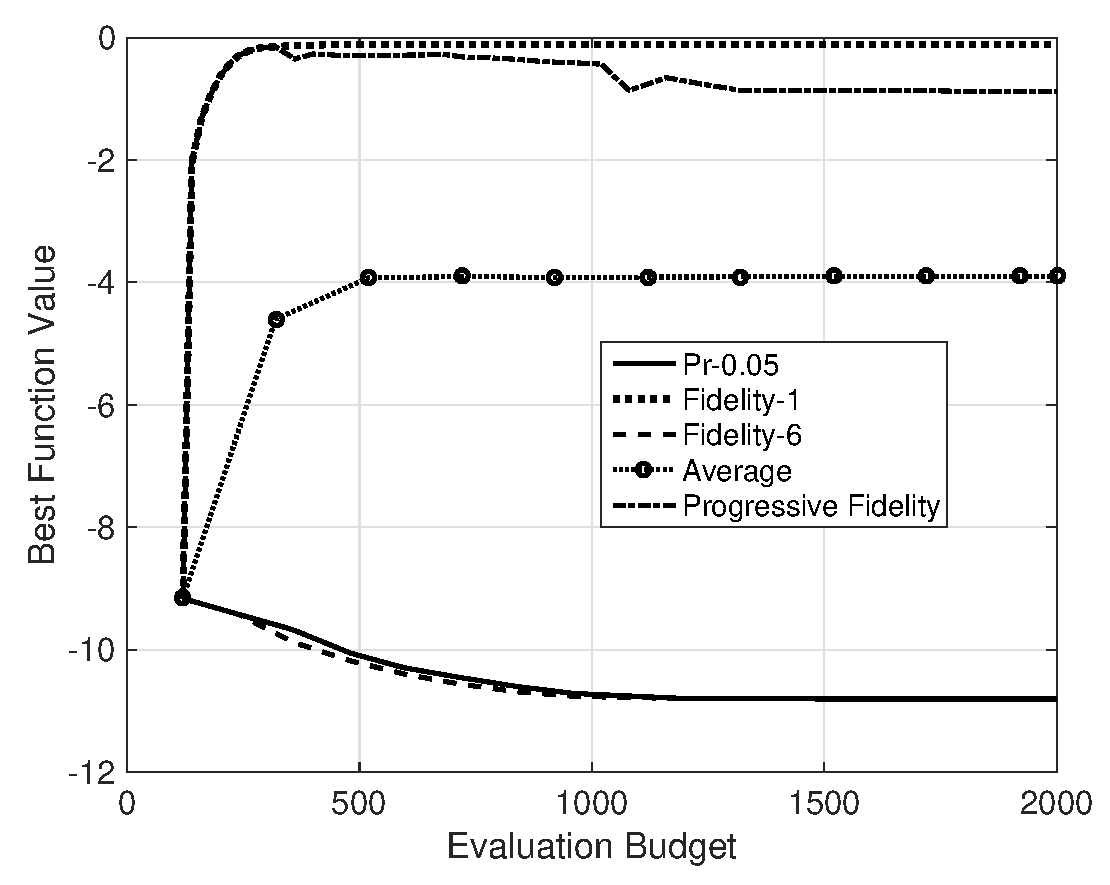
\includegraphics[width=\linewidth]{Figures/Figure17.eps}
	\caption{Convergence plot for various approaches on the PF2 test function.}
	\label{fig:pf2}
\end{figure}


\section{Conclusion}
In this paper, a novel learning based approach is introduced for the solution of optimization problems involving expensive simulation models that can be stopped early to obtain a computationally less expensive low fidelity model. Multiple logistic regression models are learned and used to rank and identify individuals in the population that can be confidently included in the next population or discarded based on partially converged simulation results. The behavior of the scheme is illustrated on two new benchmark problems: a simple artificial test function as well as a close-to-real-world higher dimensional mechanical design problem. The performance of the algorithm is compared with different single fidelity optimization strategies and a progressive fidelity strategy, and the results show that our proposed MFEA is able to produce good results independent of the available computational budget and without requiring to specify a fidelity level. It significantly outperforms alternative approaches using progressive fidelity levels or choosing the fidelity level at random.

Several extensions to the current approach seem interesting.
\begin{itemize}
	
	\item
	In the current form, the logistic regression models are built using all available data, but it would be possible to build local models instead of global models. In such a case, for every point under consideration, a number of neighboring points needs to be identified which would then be used to build the logistic regression models, better reflecting the local characteristics of the search space.
	\item
	The approach should be extended to handle also constraint problems, and even problems where the objectives and constraints may not all have the same number of fidelity levels. 
	\item
	The approach may be extended to multi-objective optimization problems. An extension along these lines would then pave the way for an easier adoption within the multidisciplinary design optimization~(MDO) community.
\end{itemize}

\begin{figure}[!htb]
\centering
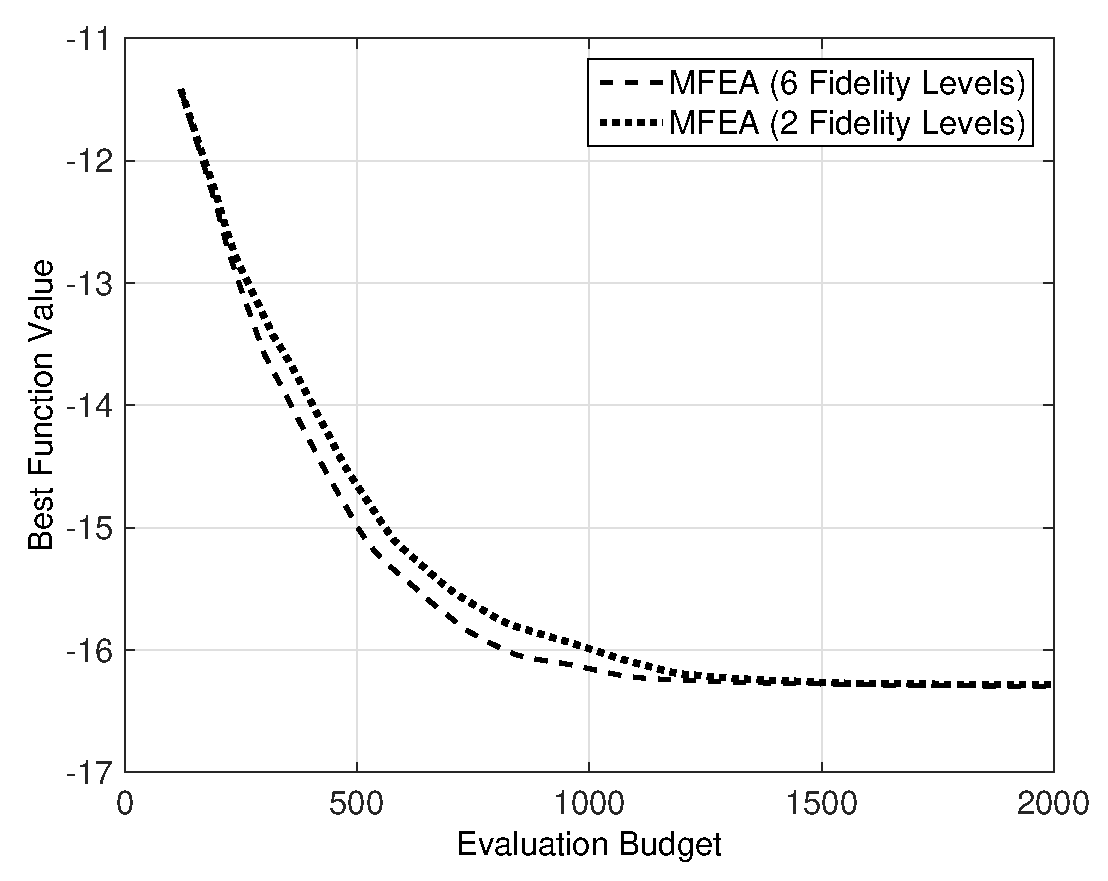
\includegraphics[width=\linewidth]{Figures/Figure18.eps}
\caption{Comparison of convergence with different number of fidelity levels without forced condition for simple test function}
\label{fig:testfidNotForcing}
\end{figure}

\begin{figure}[!htb]
\centering
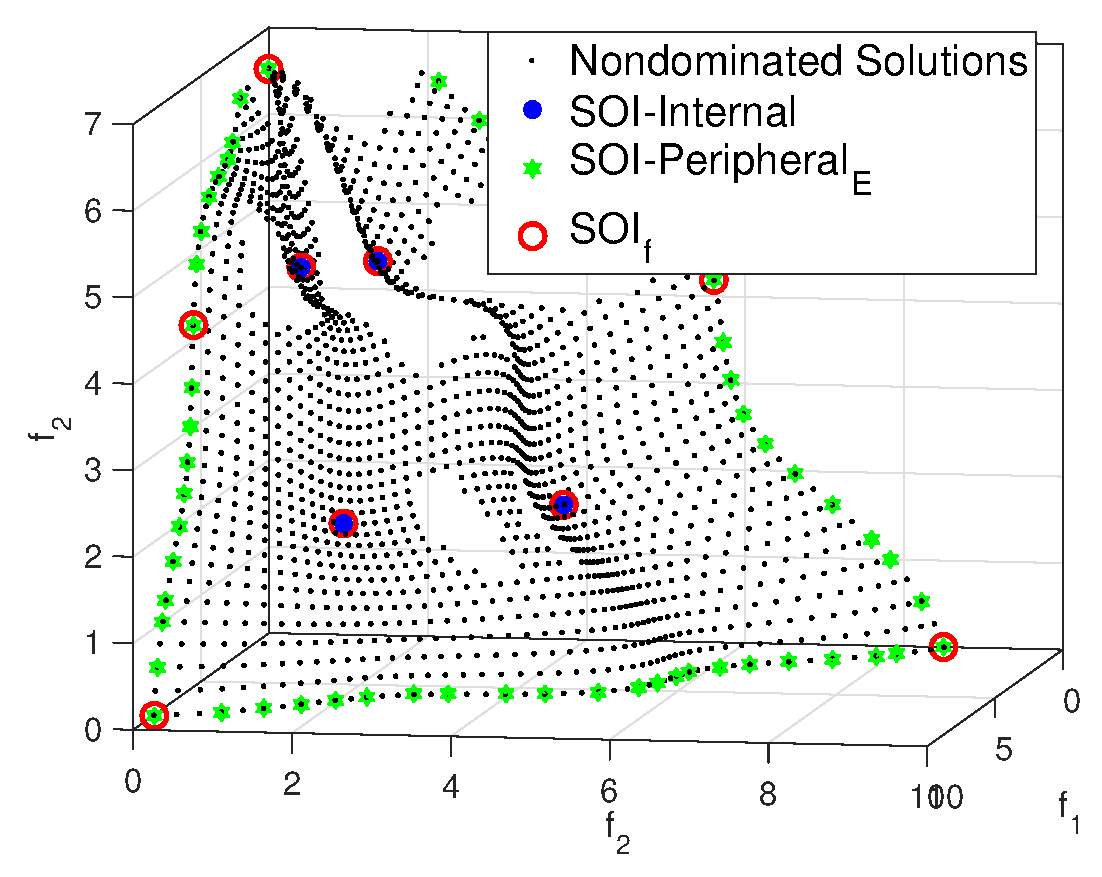
\includegraphics[width=\linewidth]{Figures/Figure19.eps}
\caption{Comparison of convergence with different number of fidelity levels without forced condition for Toysub test problem}
\label{fig:toysubfidNotForcing}
\end{figure}
